\documentclass[aspectratio=1610]{beamer}
\setbeamersize{text margin left=7mm,text margin right=5mm}
\usefonttheme[onlymath]{serif}
\usetheme{default}
\usefonttheme{professionalfonts}
%\setbeamertemplate{navigation symbols}{} 
\beamertemplatenavigationsymbolsempty
\addtobeamertemplate{navigation symbols}{}{
    \usebeamerfont{footline}
    \usebeamercolor[fg]{footline}
    %\hspace{1em}
    \small\insertframenumber\,%/\inserttotalframenumber
}


\definecolor{rcomment}{rgb}{0.3, 0.3, 0.3}  % darkgrey
\definecolor{rred}{rgb}{0.7,0.2,0.2}        % red
\definecolor{rblue}{rgb}{0.2,0.2,0.7}       % blue (blended blue of beamer)
\definecolor{rpurple}{rgb}{0.45, 0.0, 0.9}  % violett
\definecolor{rpink}{rgb}{0.8, 0.0, 0.4}     % pink
\definecolor{rgreen}{rgb}{0.1, 0.5, 0.1}    % darkgreen
\definecolor{rorange}{rgb}{0.8, 0.4,0}      % orange
\definecolor{rblack}{rgb}{0, 0, 0}          % black
\definecolor{deeptuerkis}{rgb}{0, 0.5, 0.5} % Türkis
\definecolor{darkgreen}{rgb}{0,0.5,0}
\definecolor{blendedblue}{rgb}{0.2,0.2,0.7}
\newcommand{\important}[1]{{\color{green!60!black}#1}}

% \documentclass{beamer}
% \mode<presentation> {
%   \usetheme{Singapore}
%   \setbeamertemplate{navigation symbols}{}
%   \setbeamertemplate{footline}[frame number]
% }

\usepackage[utf8]{inputenc}
\usepackage{caption}
\usepackage{nicefrac}
\usepackage{varwidth}
\usepackage{amsmath}
\usepackage{hyperref}
\usepackage{color}
\usepackage{xcolor}
\usepackage[linesnumbered, ruled, noend]{algorithm2e}
\usepackage{appendixnumberbeamer}
\usepackage{booktabs}

\usepackage{natbib}
% \usepackage[backend=bibtex,style=authoryear-comp]{biblatex}
% \bibliography{bibliography}

\usepackage[draft,nomargin,inline]{fixme}  % add final for disabling remarks
\fxsetface{inline}{\itshape}
\fxsetface{env}{\itshape}
%\fxuselayouts{margin}
%\fxuselayouts{inline}
\fxusetheme{color}

\usepackage{tikz}
\usepackage{pgfplots}
\usetikzlibrary{calc, decorations.markings}
\tikzset{vertex/.style={circle, draw=black}}
\tikzset{tr/.style={draw=white, fill=white, sloped}}
\tikzset{del/.style={draw=red, text=red}}
\tikzset{layer/.style={rectangle, draw=black, minimum width=1.5cm, minimum height=0.75cm}}
\tikzset{plus/.style={
  circle, draw=black, minimum width=0.3cm, inner sep=0cm, outer sep=0cm,
  path picture={
    \draw[black] (path picture bounding box.south) -- (path picture bounding box.north)
                 (path picture bounding box.west) -- (path picture bounding box.east);
  }
}}
\tikzset{buswidth/.style={decoration={
  markings,
  mark=at position 0.5 with {\node[font=\footnotesize] {/};\node[below=3pt] {\tiny #1};}
}, postaction={decorate}}}

\newcommand{\tmax}{\ensuremath{t^\mathrm{max}}}
\newcommand{\plim}{\ensuremath{p^\mathrm{lim}}}
\newcommand{\ILP}{\ensuremath{\mathrm{ILP}}}
\newcommand{\ppath}{\ensuremath{p^\mathrm{path}}}
\newcommand{\Tavail}{T^\mathrm{avail}}
\newcommand{\Irej}{I^\mathrm{rej}}
\newcommand{\Greedy}{\textsc{Greedy}}
\newcommand{\Markov}{\textsc{Markov}}

% \renewcommand{\thefootnote}{\fnsymbol{footnote}}

\title{Learning to Guide Heuristic Search in Combinatorial Optimization}

\author{Günther R.\ Raidl}
\date{Seminar talk at the Centre of Data Science and AI\\ Victoria University of Wellington, NZ\\March 13, 2024}
\titlegraphic{\includegraphics[height=7mm]{figures/logo-tuwien-informatics.png}\quad
	\includegraphics[height=7mm]{figures/AClongColor.pdf}}

\institute[]{Algorithms and Complexity Group, TU Wien, Austria,\\
    raidl@ac.tuwien.ac.at\\[1ex]
}

\logo{\includegraphics[height=15pt]{figures/logo.pdf}\vspace{245pt}} % Logo on top right


\definecolor{rred}{rgb}{0.7,0.2,0.2}         % red
\newcommand{\hl}[1]{\textcolor{rred}{#1}}    % highlight

\definecolor{rgreen}{rgb}{0.216,0.784,0.216} % green
\definecolor{rblue}{rgb}{0.216,0.443,0.784}  % blue
\definecolor{rorange}{rgb}{1.0,0.4,0.0}      % orange

\definecolor{orange}{RGB}{255,100,66}
\definecolor{seaborn0}{HTML}{1f77b4}
\definecolor{seaborn1}{HTML}{ff7f0e}
\definecolor{seaborn2}{HTML}{2ca02c}
\definecolor{seaborn3}{HTML}{d62728}
\definecolor{seaborn4}{HTML}{9467bd}
\definecolor{seaborn5}{HTML}{8c564b}
\definecolor{seaborn6}{HTML}{e377c2}
\definecolor{seaborn7}{HTML}{7f7f7f}
\definecolor{seaborn8}{HTML}{bcbd22}
\definecolor{seaborn9}{HTML}{17becf}

\newbool{printlegend}

\newcommand{\cumuldistr}[7]{ % Arguments: source directory, data series, width, height, x label, y label, title
  \begin{tikzpicture}
    \begin{semilogxaxis}[%
          width={#3},
          height={#4},
          title style={align=center},
          title={\large #7},
          xlabel style={at={(axis description cs:0.5,0.05)},anchor=north},
          xlabel=#5,
          ylabel style={align=center},
          ylabel=#6,
          every axis plot post/.append style={mark=none},
          every axis plot/.append style={thick},
          legend entries={GNN,Random,Sorted,Hooker},
          \ifbool{printlegend}{
            legend columns=1,
            legend pos=south east,
          }{
            legend to name=legend:cumuldistr-#1-#2,
            legend columns=-1,
          }
          ]
      \addplot+[seaborn0, solid]  table [x=#2, y=no_instances, col sep=comma, mark=none] {#1/pgdeletion_#2.csv};
      \addplot+[seaborn1, dashed] table [x=#2, y=no_instances, col sep=comma, mark=none] {#1/deletion_#2.csv};
      \addplot+[seaborn2, dashed] table [x=#2, y=no_instances, col sep=comma, mark=none] {#1/sdeletion_#2.csv};
      \addplot+[seaborn3, dashed] table [x=#2, y=no_instances, col sep=comma, mark=none] {#1/hdeletion_#2.csv};
    \end{semilogxaxis}
  \end{tikzpicture}
}

\renewcommand{\footnotesize}{\scriptsize}

\begin{document}{}


\part{Main}

\begin{frame}
  \titlepage
\end{frame}


\begin{frame}{Algorithms and Complexity Group @ TU Wien}

Part of Informatics Faculty @ TU Wien

\smallskip
5 Professors + $\approx$6 PostDoc + $\approx$25 PreDoc researchers 

\medskip
\structure{Main research areas:}

\medskip
\begin{minipage}{0.4\textwidth}
  \begin{itemize}
      \item algorithm design \& analysis
      \item combinatorial optimization
      \item complexity theory
      \item computational geometry
      \item constraint programming
      \item fixed-parameter algorithms
  \end{itemize}
\end{minipage}\qquad
\begin{minipage}{0.4\textwidth}
  \begin{itemize}
      \item graph algorithms
      \item graph drawing
      \item heuristic problem solving
      \item machine learning
      \item mathematical programming
      \item SAT solving
    \end{itemize}
  \end{minipage}

  \bigskip
  \includegraphics[width=\textwidth]{img/group.jpg}
\end{frame}


\begin{frame}{Main Research Interests of G.~R.}
    \begin{itemize}
      \item Combinatorial optimization
      \item Metaheuristics including evolutionary methods
      \item Mathematical programming
      \begin{itemize}
        \item incl.\ mixed-integer linear programming, column generation, branch-and-cut-and-price, (logic-)based Benders decomposition
      \end{itemize}
      \item Constraint programming
      \item Machine learning
      \item \important{\bf Hybrid approaches} incl.\ matheuristics, learning + classical algorithms for COP
    \end{itemize} 
    
    \vspace{0.3cm}
    \structure{Application areas:}
    \begin{itemize}
      \item Transport optimization
      \item Scheduling
      \item Network design
      \item Problems in bioinformatics
      \item Cutting and packing
    \end{itemize}
\end{frame}

\begin{frame}{Selected Ongoing Projects}
\begin{itemize}
  \itemsep3.5ex
  \item Dynamic Vehicle Routing Problems with Focus on E-mobility \& Learning
  \begin{itemize}
    \item with T.~Rodemann et al., Honda Research Institute Europe
  \end{itemize}
  \item Cooperative Personnel Scheduling
  \begin{itemize}
    \item with S.~Limmer et al., Honda Research Institute Europe
  \end{itemize}
  \item Doctoral College Vienna Graduate School on Computational Optimization
  \begin{itemize}
    \item with University of Vienna, IST Austria, Vienna University of Economics and Business
  \end{itemize}
  \item Solving Roman Domination Problems, Influence Maximization Problems, and Variants
  \begin{itemize}
    \item with M. Djukanovic et al., Univ.\ of Banja Luka, Bosnia and Herzegovina
  \end{itemize}
\end{itemize}
\end{frame}



\begin{frame}{Combinatorial Optimization and Learning}
	\begin{itemize}
		\itemsep2.5ex
		\item \important{AI/machine learning boom} also hit the area of \important{combinatorial optimization}
		\item This in many different ways
		\begin{center}
			\centering
			\includegraphics[width=0.85\linewidth]{figures/mh-ml}
		\end{center}
		\item \structure{Focus here:} utilize learning to better solve \important{combinatorial optimization problems (COPs)}
		\item \alert{Basic idea of learning in MHs not new!}
	\end{itemize}
\end{frame}


\begin{frame}{Learning to Better Optimize}
	\begin{center}
		\includegraphics[width=0.95\linewidth]{figures/talbi-data-driven-mhs}\\[2ex]
		\footnotesize{(from \citet{talbi-21})}
	\end{center}
\end{frame}


\begin{frame}{Some Classical Metaheuristics Involving Learning}
    \begin{itemize}
    \itemsep2.5ex
	%\item Simulated Annealing with self-adaptive temperature
	
	\item Reactive tabu search
	\item Evolution Strategies
	\item Guided Local Search 
	\item Variable Neighborhood Search, \\
	Adaptive Large Neighborhood Search
	\begin{itemize}
		\item self-adaptive selection of neighborhood structures/operators
	\end{itemize}
	\item Hyper-heuristics
	%\item<2> \important{Monte Carlo Tree Search}
	\item Ant Colony Optimization
  \end{itemize}
\end{frame}


\begin{frame}{Idea of Ant Colony Optimization}
	\begin{itemize}
		\item Iteratively construct solutions in a randomized greedy fashion
		\item Additionally consider \important{pheromone values}:
		\item Decisions in good solutions are \important{reinforced} by increasing their pheromone values while other values are reduced by ``evaporation''
	\end{itemize}
	\begin{center}
		\includegraphics[width=0.4\linewidth]{figures/aco} \\
		{\footnotesize (from Dr\'eo, 2006)}

    \bigskip
    \important{\bf $\rightarrow$ Similarities with Reinforcement Learning!}
	\end{center}
\end{frame}

% \begin{frame}{Some Classical (Meta)heuristics Involving Learning}
% 	\begin{itemize}
% 		\itemsep2.5ex
% 		%\item Simulated Annealing with self-adaptive temperature
% 		\item Variable Neighborhood Search, \\
% 		Adaptive Large Neighborhood Search
% 		\item Evolution Strategies
% 		\begin{itemize}
% 			\item self-adaptive selection of neighborhood structures/operators
% 		\end{itemize}
% 		\item Guided Local Search 
% 		\item Reactive Tabu Search

% 		\item Ant Colony Optimization
% 		% \item Hyper-heuristics
% 	\end{itemize}
% \end{frame}





% \begin{frame}{Idea of Monte Carlo Tree Search (MCTS)}
% 	\begin{itemize}
% 	\item Originates from playing board games, e.g., Go, Chess
% 	\item Info stored in nodes: \important{\# of wins / \# of visits}
% 	\item Four phases, repeated as long as there is time left:
% 	\end{itemize}
% 	\begin{center}
% 		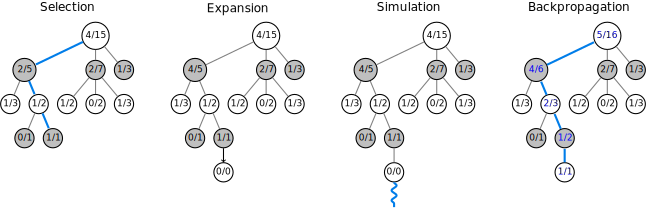
\includegraphics[width=0.9\linewidth]{figures/MCTS2.pdf}
% 	\end{center}
% 	\vspace{-3ex}
% 	\begin{itemize}
% 	\item\only<1>{\important{Selection}: 
% 	\begin{itemize}
% 		\item traverse tree from the root until leaf reached
% 		\item always select successor that maximizes e.g.\ the UCT criterion: 
% 			$\mathit{UCT}_j = \frac{\#\mathit{wins}_j}{\#\mathit{visits}_j} + c\cdot\sqrt{\frac{\ln \#\mathit{visits}_{i}}{\#\mathit{visits}_j}}$ for successor $j$ of node $i$
% 	\end{itemize}}
% 	\only<2>{\important{Expansion}:
% 		\begin{itemize}
% 			\item add new leaf node
% 		\end{itemize}}
% 	\only<3>{\important{Simulation}: 
% 		\begin{itemize}
% 			\item perform self-play until end of game, e.g., by random rollout
% 			\item result is either 1, 0, or -1
% 		\end{itemize}}
% 	\only<4>{\important{Backpropagation}: 
% 		\begin{itemize}
% 			\item Update visit and win counters on all nodes up to the root
% 		\end{itemize}}
% 	\end{itemize}
	
% \end{frame}

% \begin{frame}{Survey Articles}
% 	\begin{itemize}
% 		\itemsep2ex
% 		\item M.~Karimi-Mamaghan et al.: \emph{Machine Learning at the Service of Metaheuristics for solving COPs: A State-of-the Art}; EJOR, 2021
% 		\item E.-G.~Talbi: \emph{Machine Learning into Metaheuristics: A Survey and Taxonomy}; ACM Computing Surveys, 2021
% 		\item N.~Mazyavkina et al.: \emph{Reinforcement Learning for Combinatorial Optimization: A Survey}; COR, 2021
% 	\end{itemize}
% \end{frame}

\begin{frame}{Learning to Better Optimize}
	\begin{center}
		\includegraphics[width=0.75\linewidth]{figures/talbi-data-driven-mhs}\\[2ex]
		\footnotesize{From \citet{talbi-21}: Machine Learning into Metaheuristics: A Survey and Taxonomy}
	\end{center}
\end{frame}

% \begin{frame}{High-Level Data Driven Metaheuristics}
% %Idea of \textbf{using some kind of \important{learning} to better solve an optimization problem} at hand is not new.

% %\medskip
% % Well established are also:

% \medskip
% \begin{itemize}
% 	\itemsep2ex
% 	\item \structure{Automated Algorithm Selection}
% 	\begin{itemize}
% 		\item From an algorithm portfolio, select for a given problem instance a best suited algorithm based on features of the instance
% 		\begin{center}
% 			\includegraphics[width=0.7\linewidth]{figures/alg-selection}
% 		\end{center}
		
% 	\end{itemize}
% 	\item \structure{Automated Algorithm Configuration}
% 		\begin{itemize}
% 		\item Select components and parameters of an algorithm based on instance features
% 	\end{itemize}
% \end{itemize}
% \end{frame}

% \begin{frame}{Learning to Better Optimize}
% \begin{center}
% 	\includegraphics[width=0.95\linewidth]{figures/talbi-data-driven-mhs}\\[2ex]
% 	\footnotesize{(from Talbi, 2020: Machine Learning in Metaheuristics)}
% \end{center}
% \end{frame}

% \begin{frame}{Learning to Better Optimize}
% 	\begin{center}
% 		\includegraphics[width=0.95\linewidth]{figures/talbi-data-driven-objective-functions}\\[2ex]
% 		\footnotesize{(from Talbi, 2020: Machine Learning in Metaheuristics)}
% 	\end{center}
% \end{frame}

% \begin{frame}{Learning to Better Optimize}
% 	\begin{center}
% 		\includegraphics[width=0.95\linewidth]{figures/talbi-data-driven-constraints}\\[2ex]
% 		\footnotesize{(from Talbi, 2020: Machine Learning in Metaheuristics)}
% 	\end{center}
% \end{frame}



\begin{frame}{Reinforcement Learning (RL)}
	\begin{itemize}
		\item A sub-discipline of machine learning
		\item Environment is usually considered a \structure{Markov decision process}
		%\item Received much attention in broader public by DeepMind's successes in agents for Go, chess, and diverse video games
		\item Framework:\\
		\begin{minipage}[c]{0.45\textwidth}
			\includegraphics[width=\linewidth]{figures/reinforcement_learning}
		\end{minipage} \hfill
		\begin{minipage}[c]{0.20\textwidth}
		% \begin{textblock}{20}(40,20)
			\includegraphics[width=\linewidth]{figures/cartpole.png}\\[1cm]
			%\includegraphics[width=3cm]{figures/compgames.jpg}\\
			\includegraphics[width=\linewidth]{figures/alphazero.png}
		\end{minipage}
		\begin{minipage}[c]{0.20\textwidth}
			% \begin{textblock}{20}(40,20)
				\includegraphics[width=\linewidth]{figures/compgames.jpg}
			\end{minipage}

		\vspace{2ex}
		\item<2> \alert{Constructing a solution to a COP can be seen as an episode in an environment, objective value $\hat=$ reward}
	\end{itemize}
\end{frame}


\begin{frame}
	\frametitle{Reinforcement Learning (RL) - Classification}
	\begin{center}
		\includegraphics[width=0.8\textwidth]{figures/rlmethods.jpg}

		\bigskip
		\footnotesize{(from \citet{mazyavkina-21b})}
	\end{center}
\end{frame}


% \begin{frame}{Q-Learning \citep{watkins1992q}}
% 	\begin{itemize}
% 		\itemsep2ex
% 		\item model-free, for discrete state and action spaces, off-policy
% 		\item \structure{Goal:} max.\ weighted sum of expected rewards for all future steps
		
% 		\item Table with \important{Q-value $Q(s,a)$} for each state/action pair $(s,a)$:\\
% 		approximates expected weighted sum of rewards to receive from state $s$ onward when performing action $a$
% 		\item Update of initially random $Q(s,a)$ values by\\
% 		\begin{center}
% 			\includegraphics[width=1\linewidth]{figures/q-learning-equation}
% 		\end{center}
% 		% $Q(s_t,a_t) \leftarrow Q(s_t,a_t) + \alpha \left( R_{t+1} + \gamma\max_{a} Q(s_{t+1},a) - Q(s_t,a_t)\right)$
% 		\item<2->{\important{Compare Q-Learning and Ant Colony Optimization!}}
% 		\item<3-> Frequently too many states $\rightarrow$ approximate $Q(s,a)$ by a (deep) neural network $\rightarrow$ \important{Deep Q Network} (DQN, Mnih et al., 2013)
% 	\end{itemize}
% \end{frame}

% \begin{frame}{Reinforcement Learning (RL)}
% 	\begin{itemize}
% 		\itemsep1.5ex
% 		% \item Ant colony optimization, MCTS can be said to be RL agents
% 		\item Many different RL agents have been proposed in recent years
% 		\item Agents differ in
% 		\begin{itemize}
% 			\item state space (discrete/continuous)
% 			\item action space (discrete/continuous)
% 			\item on-policy/off-policy
% 			\item model-free/model-based
% 		\end{itemize}
% 		\important{Deep} RL: uses deep neural networks
% 		\item Examples of agents: Q-Learning, SARSA, DQN, DDPG, A3C, TRPO, PPO, SAC, \ldots 
% 	\end{itemize}
% \end{frame}

% \begin{frame}
% 	\frametitle{RL for Combinatorial Optimization -- Classification}

% 	according to \citet{mazyavkina-21b}:

% 	\vspace{1cm}
% 	\begin{itemize}
% 	 	\itemsep2ex
% 		\item \structure{Principal learning:}\\ agent makes direct decisions to construct solution
% 		\begin{itemize}
% 			\item ``end-to-end'' learning
% 			\item usually far from competitive to classical state-of-the art methods in combinatorial optimization
% 		\end{itemize}
% 		\item \structure{Joint approach:}\\ agent works jointly with some classical solver/algorithm
% 		\begin{itemize}
% 			\item agent ``helps/guides'' classical solver in some way
% 			\item agent learns from classical solver (\important{imitation learning})
% 		\end{itemize}
% 		\vspace{8mm}
% 		\item \structure{Construction based} vs.\ \structure{improvement based}
% 	\end{itemize}
% \end{frame}


\begin{frame}
	\frametitle{Encoding of Problems+States, ML Models}

	\begin{itemize}
		\itemsep3ex
		\item encoding highly problem-specific
		\item variants of (deep) neural networks dominate the used ML models
		\begin{itemize}
			\itemsep1.3ex
			\item recurrent neural networks, e.g., LSTMs
			% \item attention models
			\item \structure{pointer networks} \citep{vinyals-2015}
			\item variants of \structure{Graph Neural Networks} \citep{scarselli2008graph}, e.g.,
			\begin{itemize}
				\item Structure-to-Vector Network (Dai et al., 2016)
				\item Graph Convolutional Network (Kipf and Welling, 2017)
				\item Graph Isomorphism Network (Xu et al., 2019)
				\item Graph Attention Network (Kool et al., 2019; Joshi et al., 2021)
			\end{itemize}
			{\includegraphics[width=0.7\linewidth, page=3]{figures/graphics.pdf}}\\
			% learn \important{embedding of nodes} by looking at nearby nodes
		\end{itemize} 
	\end{itemize}
\end{frame}

\begin{frame}{Learning to Solve Graph Problems}
	\begin{itemize}
		\itemsep2ex
		\item \structure{\citet{dai-17}}: \important{S2V-DQN}
		\item min vertex cover, max cut, TSP considered 
		\item graph embedding network \important{structure2vec} used to ``featurize'' nodes
		\item variant of Q-learning used to obtain a policy for greedily constructing solutions
		\begin{center}
			\includegraphics[width=1\linewidth]{figures/dai}
		\end{center}
	\end{itemize}
\end{frame}

% \begin{frame}{Learning to Solve Graph Problems (cont.)}
% 	\begin{itemize}
% 		\itemsep1.5ex
% 		\item \structure{\citet{mittal-19}}: \important{GCOMB}
% 		\item focus on scalability to graphs with millions of nodes\\ max influence, max vertex cover, max coverage problems considered
% 		\item \important{GCN} trained in supervised fashion to predict likelihood of each node to be part of a solution
% 		\item \important{Q-learning} finds combination of most promising nodes\\
% 		$Q(S,v)$: long-term reward for adding node $v$ to solution $S$\\ approximated by a comparatively simple neural net
% 		\begin{center}
% 			\includegraphics[width=1\linewidth]{figures/mittal}
% 		\end{center}
% 	\end{itemize}
% \end{frame}

\begin{frame}{Learning to Solve Graph Problems (cont.)}
	\begin{itemize}
		\item \structure{\citet{kool-19a}}
		\item Autoregressive multi-head attention-based encoder/decoder GNN
		\item for TSP, VRP
		\begin{center}
			\includegraphics[width=0.7\linewidth]{figures/MHA-encoder.jpg}
		\end{center}
		\begin{center}
			\includegraphics[width=0.7\linewidth]{figures/MHA-decoder.jpg}
		\end{center}
		\item Trained with REINFORCE
	\end{itemize}
\end{frame}

\begin{frame}{Learning to Solve Graph Problems (cont.)}
\begin{itemize}
	\itemsep1ex
	\item \structure{\citet{li-18}}
	\item max independent set, min vertex cover, max clique, SAT considered
	\item \important{Graph Convolutional Network (GCN)} used to predict likelihood of each node to be part of a solution
	\item GCN yields \important{multiple probability maps} to account for the fact that multiple optimal solutions may exist
	\item \important{heuristic tree search} utilizing multiple maps,\\ \important{graph reduction, basic local search} applied
	\item \important{supervised learning} instead of reinforcement learning
	\item results competitive to state-of-the-art solvers reported 
	\medskip
	\begin{center}
		\includegraphics[width=1\linewidth]{figures/li}
	\end{center}
\end{itemize}
\end{frame}

% \begin{frame}{Basic Idea of AlphaGoZero \citep{silver-18}}
% 	\begin{itemize}
% 		\item Superhuman agent for Go, successor of AlphaGo
% 		\item Learns only by \important{iterated selfplay}:\\
% 		%\begin{center}
% 			\includegraphics[width=0.9\linewidth]{figures/alpha-zero-selfplay}
% 		%\end{center}
% 		\item \important{Monte Carlo Tree Search (MCTS)} is applied to obtain a policy and select a move
% 		\item \important{In the MCTS new states are evaluated by a deep neural net}:
% 		\begin{itemize}
% 			\item input: board state
% 			\item output: \important{policy}, i.e., probabilities for all positions; \important{value}, i.e., probability to win
% 		\end{itemize}
% 		\item \important{Neural net output is \textbf{boosted} by MCTS!}
% 	\end{itemize}
% \end{frame}

% \begin{frame}{Basic Idea of AlphaGoZero \citep{silver-18}}
% 	\begin{center}
% 	\includegraphics[width=1\linewidth]{figures/alpha-zero-training}
% 	\end{center}
% 	\begin{itemize}
% 		\item selfplay games are logged with results in a \important{replay buffer}
% 		\item neural net continuously trained with samples from replay buffer
% 	\end{itemize}
% \end{frame}

\begin{frame}{Learning to Solve Graph Problems}
	\begin{itemize}
		\itemsep1.1ex
		\item \structure{\citet{abe-20}}: \important{CombOptZero}
		\item min vertex cover, max cut, max clique problems considered
		\item based on the principles of \important{AlphaGoZero}
		\item \important{different graph neural networks} tested, including GCN
		\item special reward normalization applied
		\item outperforms S2V-DQN, results close to state-of-the-art reported
		
		% \vspace{3ex}
		% \item \structure{\citet{huang-19}}: similar approach for \important{coloring large graphs} with millions of nodes
		% \item special \important{FastColorNet} neural network architecture
		% \item claimed to yield new state-of-the-art results
	\end{itemize}
\end{frame}


% \begin{frame}
% 	\frametitle{Learning Beam Search \citep{huber-21}}
% 	\medskip
% 	\structure{Beam Search (BS)}: Breadth-First-Search, in which at each level only $\beta$ most promising nodes are kept; $\beta$: beam width

% 	\bigskip
% 	\onslide<1>{
% 	\structure{Learning Beam Search (LBS)}
% 	\begin{itemize}
% 		\itemsep2ex
% 		\item Initialize ML model \important{$h_{\Theta}(v)$} for the value of evaluating nodes $v$ randomly
% 		\item Iterate:
% 		\begin{itemize}
% 			\itemsep1.5ex
% 			\item Create a random problem instance
% 			\item Perform a BS, guided by the ML model
% 				\begin{itemize}
% 					\item From each non-terminal node $v$ with small probability:
% 					\item[\qquad--] Perform a \important{Nested BS (NBS)} to obtain a training sample
% 					\item[\qquad--] Store training sample in a limited size FIFO \important{replay buffer}
% 				\end{itemize}
% 			\item (Re-)train ML model on samples from replay buffer.
% 		\end{itemize}
% 	\end{itemize}}
% 	% \begin{enumerate}
% 	% 	\item , where \medskip
% 	% 		\begin{itemize}
% 	% 			\item Input: Problem-specific feature vector that captures relevant information from the state of a node $v$ and the problem instance.
% 	% 				\medskip
% 	% 			\item Output: $h(v)$ = estimated further length to go from $v$.
									
% 	% 		\end{itemize}

% 	% 	\item Repeat steps 2-4 until a stopping criterion is fulfilled.
% 	% \end{enumerate} 
% \end{frame}

	
\begin{frame}
\frametitle{Learning Beam Search \citep{huber-21}}
	\begin{center}
		\includegraphics[height=210pt]{figures/lbsProcedure.png}
	\end{center}
\end{frame}
	
% \begin{frame}%[t,c,b,plain]
% 	\frametitle{LBS Experiments: Considered Problems}
	
% 	\medskip
	
% 	\structure{Given:} set of $m$ input strings $S = \{s_1 , \ldots, s_m \}$ over alphabet $\Sigma$.
	
% 	\medskip
	
% 	\begin{itemize}
% 		\item \structure{Longest Common Subsequence (LCS):} find a longest string that appears as subsequence in any string of $S$. \\ \medskip
% 		Example: $m=2$, $|\Sigma|=3$
% 	\end{itemize}
% 	\begin{center}
% 	\begin{tabular}{ccc}
% 		$s_1$: AB\textcolor{gray}{B}A & \multirow{2}{*}{$\Rightarrow$ \textcolor{red}{ABA}.}\\
% 		$s_2$: \textcolor{gray}{C}ABA
% 	\end{tabular}
% 	\end{center}
	
% 	% \begin{itemize}
% 	% 	\item \structure{Constrained Longest Common Subsequence (CLCS):} additionally, a pattern string $P$ must appear as subsequence. \\ \medskip
% 	% 	Example: P=\textcolor{darkgreen}{AB}
% 	% \end{itemize}
% 	% \begin{center}
% 	% \begin{tabular}{ccc}
% 	% 	$s_1$: AB\textcolor{gray}{B}A & \multirow{2}{*}{$\Rightarrow$ \textcolor{darkgreen}{AB}A.}\\
% 	% 	$s_2$: \textcolor{gray}{C}ABA
% 	% \end{tabular}
% 	% \end{center}

% 	\bigskip
% 	\structure{State-of-the-art:} BS with theoretically derived guidance functions EX \citep{djukanovic-19b}
% \end{frame}

% \begin{frame}
% 	\frametitle{LBS Experiments: Approximation of Real LCS Length}
% 	% \bigskip
% 	% \textbf{How well does a NN trained by LBS predict the real LCS length?}
% 	% \medskip
% 	% \begin{itemize}
% 	% 	\item Approximate exact LCS lengths by applying the so far leading BS with EX guidance function~\citep{djukanovic-19b}.
% 	% \end{itemize}
	
% 	The NN of the LBS approximates the real LCS lengths better than EX:

% 	\bigskip
% 	\begin{center}
% 		% \makebox[\linewidth]{
% 		%% Creator: Matplotlib, PGF backend
%%
%% To include the figure in your LaTeX document, write
%%   \input{<filename>.pgf}
%%
%% Make sure the required packages are loaded in your preamble
%%   \usepackage{pgf}
%%
%% and, on pdftex
%%   \usepackage[utf8]{inputenc}\DeclareUnicodeCharacter{2212}{-}
%%
%% or, on luatex and xetex
%%   \usepackage{unicode-math}
%%
%% Figures using additional raster images can only be included by \input if
%% they are in the same directory as the main LaTeX file. For loading figures
%% from other directories you can use the `import` package
%%   \usepackage{import}
%%
%% and then include the figures with
%%   \import{<path to file>}{<filename>.pgf}
%%
%% Matplotlib used the following preamble
%%
\begingroup%
\makeatletter%
\begin{pgfpicture}%
\pgfpathrectangle{\pgfpointorigin}{\pgfqpoint{4.200000in}{1.350000in}}%
\pgfusepath{use as bounding box, clip}%
\begin{pgfscope}%
\pgfsetbuttcap%
\pgfsetmiterjoin%
\definecolor{currentfill}{rgb}{1.000000,1.000000,1.000000}%
\pgfsetfillcolor{currentfill}%
\pgfsetlinewidth{0.000000pt}%
\definecolor{currentstroke}{rgb}{0.500000,0.500000,0.500000}%
\pgfsetstrokecolor{currentstroke}%
\pgfsetdash{}{0pt}%
\pgfpathmoveto{\pgfqpoint{0.000000in}{0.000000in}}%
\pgfpathlineto{\pgfqpoint{4.200000in}{0.000000in}}%
\pgfpathlineto{\pgfqpoint{4.200000in}{1.350000in}}%
\pgfpathlineto{\pgfqpoint{0.000000in}{1.350000in}}%
\pgfpathclose%
\pgfusepath{fill}%
\end{pgfscope}%
\begin{pgfscope}%
\pgfsetbuttcap%
\pgfsetmiterjoin%
\definecolor{currentfill}{rgb}{0.898039,0.898039,0.898039}%
\pgfsetfillcolor{currentfill}%
\pgfsetlinewidth{0.000000pt}%
\definecolor{currentstroke}{rgb}{0.000000,0.000000,0.000000}%
\pgfsetstrokecolor{currentstroke}%
\pgfsetstrokeopacity{0.000000}%
\pgfsetdash{}{0pt}%
\pgfpathmoveto{\pgfqpoint{0.377122in}{0.400271in}}%
\pgfpathlineto{\pgfqpoint{1.933738in}{0.400271in}}%
\pgfpathlineto{\pgfqpoint{1.933738in}{1.106750in}}%
\pgfpathlineto{\pgfqpoint{0.377122in}{1.106750in}}%
\pgfpathclose%
\pgfusepath{fill}%
\end{pgfscope}%
\begin{pgfscope}%
\pgfsetbuttcap%
\pgfsetroundjoin%
\definecolor{currentfill}{rgb}{0.000000,0.000000,0.000000}%
\pgfsetfillcolor{currentfill}%
\pgfsetlinewidth{0.803000pt}%
\definecolor{currentstroke}{rgb}{0.000000,0.000000,0.000000}%
\pgfsetstrokecolor{currentstroke}%
\pgfsetdash{}{0pt}%
\pgfsys@defobject{currentmarker}{\pgfqpoint{0.000000in}{-0.048611in}}{\pgfqpoint{0.000000in}{0.000000in}}{%
\pgfpathmoveto{\pgfqpoint{0.000000in}{0.000000in}}%
\pgfpathlineto{\pgfqpoint{0.000000in}{-0.048611in}}%
\pgfusepath{stroke,fill}%
}%
\begin{pgfscope}%
\pgfsys@transformshift{0.571699in}{0.400271in}%
\pgfsys@useobject{currentmarker}{}%
\end{pgfscope}%
\end{pgfscope}%
\begin{pgfscope}%
\definecolor{textcolor}{rgb}{0.000000,0.000000,0.000000}%
\pgfsetstrokecolor{textcolor}%
\pgfsetfillcolor{textcolor}%
\pgftext[x=0.571699in,y=0.303049in,,top]{\color{textcolor}\fontsize{5.800000}{6.960000}\selectfont 10}%
\end{pgfscope}%
\begin{pgfscope}%
\pgfsetbuttcap%
\pgfsetroundjoin%
\definecolor{currentfill}{rgb}{0.000000,0.000000,0.000000}%
\pgfsetfillcolor{currentfill}%
\pgfsetlinewidth{0.803000pt}%
\definecolor{currentstroke}{rgb}{0.000000,0.000000,0.000000}%
\pgfsetstrokecolor{currentstroke}%
\pgfsetdash{}{0pt}%
\pgfsys@defobject{currentmarker}{\pgfqpoint{0.000000in}{-0.048611in}}{\pgfqpoint{0.000000in}{0.000000in}}{%
\pgfpathmoveto{\pgfqpoint{0.000000in}{0.000000in}}%
\pgfpathlineto{\pgfqpoint{0.000000in}{-0.048611in}}%
\pgfusepath{stroke,fill}%
}%
\begin{pgfscope}%
\pgfsys@transformshift{0.960853in}{0.400271in}%
\pgfsys@useobject{currentmarker}{}%
\end{pgfscope}%
\end{pgfscope}%
\begin{pgfscope}%
\definecolor{textcolor}{rgb}{0.000000,0.000000,0.000000}%
\pgfsetstrokecolor{textcolor}%
\pgfsetfillcolor{textcolor}%
\pgftext[x=0.960853in,y=0.303049in,,top]{\color{textcolor}\fontsize{5.800000}{6.960000}\selectfont 40}%
\end{pgfscope}%
\begin{pgfscope}%
\pgfsetbuttcap%
\pgfsetroundjoin%
\definecolor{currentfill}{rgb}{0.000000,0.000000,0.000000}%
\pgfsetfillcolor{currentfill}%
\pgfsetlinewidth{0.803000pt}%
\definecolor{currentstroke}{rgb}{0.000000,0.000000,0.000000}%
\pgfsetstrokecolor{currentstroke}%
\pgfsetdash{}{0pt}%
\pgfsys@defobject{currentmarker}{\pgfqpoint{0.000000in}{-0.048611in}}{\pgfqpoint{0.000000in}{0.000000in}}{%
\pgfpathmoveto{\pgfqpoint{0.000000in}{0.000000in}}%
\pgfpathlineto{\pgfqpoint{0.000000in}{-0.048611in}}%
\pgfusepath{stroke,fill}%
}%
\begin{pgfscope}%
\pgfsys@transformshift{1.350007in}{0.400271in}%
\pgfsys@useobject{currentmarker}{}%
\end{pgfscope}%
\end{pgfscope}%
\begin{pgfscope}%
\definecolor{textcolor}{rgb}{0.000000,0.000000,0.000000}%
\pgfsetstrokecolor{textcolor}%
\pgfsetfillcolor{textcolor}%
\pgftext[x=1.350007in,y=0.303049in,,top]{\color{textcolor}\fontsize{5.800000}{6.960000}\selectfont 100}%
\end{pgfscope}%
\begin{pgfscope}%
\pgfsetbuttcap%
\pgfsetroundjoin%
\definecolor{currentfill}{rgb}{0.000000,0.000000,0.000000}%
\pgfsetfillcolor{currentfill}%
\pgfsetlinewidth{0.803000pt}%
\definecolor{currentstroke}{rgb}{0.000000,0.000000,0.000000}%
\pgfsetstrokecolor{currentstroke}%
\pgfsetdash{}{0pt}%
\pgfsys@defobject{currentmarker}{\pgfqpoint{0.000000in}{-0.048611in}}{\pgfqpoint{0.000000in}{0.000000in}}{%
\pgfpathmoveto{\pgfqpoint{0.000000in}{0.000000in}}%
\pgfpathlineto{\pgfqpoint{0.000000in}{-0.048611in}}%
\pgfusepath{stroke,fill}%
}%
\begin{pgfscope}%
\pgfsys@transformshift{1.739161in}{0.400271in}%
\pgfsys@useobject{currentmarker}{}%
\end{pgfscope}%
\end{pgfscope}%
\begin{pgfscope}%
\definecolor{textcolor}{rgb}{0.000000,0.000000,0.000000}%
\pgfsetstrokecolor{textcolor}%
\pgfsetfillcolor{textcolor}%
\pgftext[x=1.739161in,y=0.303049in,,top]{\color{textcolor}\fontsize{5.800000}{6.960000}\selectfont 200}%
\end{pgfscope}%
\begin{pgfscope}%
\definecolor{textcolor}{rgb}{0.000000,0.000000,0.000000}%
\pgfsetstrokecolor{textcolor}%
\pgfsetfillcolor{textcolor}%
\pgftext[x=1.155430in,y=0.173419in,,top]{\color{textcolor}\fontsize{6.960000}{8.352000}\selectfont \(\displaystyle m\)}%
\end{pgfscope}%
\begin{pgfscope}%
\pgfpathrectangle{\pgfqpoint{0.377122in}{0.400271in}}{\pgfqpoint{1.556616in}{0.706479in}}%
\pgfusepath{clip}%
\pgfsetrectcap%
\pgfsetroundjoin%
\pgfsetlinewidth{0.803000pt}%
\definecolor{currentstroke}{rgb}{1.000000,1.000000,1.000000}%
\pgfsetstrokecolor{currentstroke}%
\pgfsetdash{}{0pt}%
\pgfpathmoveto{\pgfqpoint{0.377122in}{0.400271in}}%
\pgfpathlineto{\pgfqpoint{1.933738in}{0.400271in}}%
\pgfusepath{stroke}%
\end{pgfscope}%
\begin{pgfscope}%
\pgfsetbuttcap%
\pgfsetroundjoin%
\definecolor{currentfill}{rgb}{0.000000,0.000000,0.000000}%
\pgfsetfillcolor{currentfill}%
\pgfsetlinewidth{0.803000pt}%
\definecolor{currentstroke}{rgb}{0.000000,0.000000,0.000000}%
\pgfsetstrokecolor{currentstroke}%
\pgfsetdash{}{0pt}%
\pgfsys@defobject{currentmarker}{\pgfqpoint{-0.048611in}{0.000000in}}{\pgfqpoint{0.000000in}{0.000000in}}{%
\pgfpathmoveto{\pgfqpoint{-0.000000in}{0.000000in}}%
\pgfpathlineto{\pgfqpoint{-0.048611in}{0.000000in}}%
\pgfusepath{stroke,fill}%
}%
\begin{pgfscope}%
\pgfsys@transformshift{0.377122in}{0.400271in}%
\pgfsys@useobject{currentmarker}{}%
\end{pgfscope}%
\end{pgfscope}%
\begin{pgfscope}%
\definecolor{textcolor}{rgb}{0.000000,0.000000,0.000000}%
\pgfsetstrokecolor{textcolor}%
\pgfsetfillcolor{textcolor}%
\pgftext[x=0.146414in, y=0.371336in, left, base]{\color{textcolor}\fontsize{5.800000}{6.960000}\selectfont \(\displaystyle {0.0}\)}%
\end{pgfscope}%
\begin{pgfscope}%
\pgfpathrectangle{\pgfqpoint{0.377122in}{0.400271in}}{\pgfqpoint{1.556616in}{0.706479in}}%
\pgfusepath{clip}%
\pgfsetrectcap%
\pgfsetroundjoin%
\pgfsetlinewidth{0.803000pt}%
\definecolor{currentstroke}{rgb}{1.000000,1.000000,1.000000}%
\pgfsetstrokecolor{currentstroke}%
\pgfsetdash{}{0pt}%
\pgfpathmoveto{\pgfqpoint{0.377122in}{0.577825in}}%
\pgfpathlineto{\pgfqpoint{1.933738in}{0.577825in}}%
\pgfusepath{stroke}%
\end{pgfscope}%
\begin{pgfscope}%
\pgfsetbuttcap%
\pgfsetroundjoin%
\definecolor{currentfill}{rgb}{0.000000,0.000000,0.000000}%
\pgfsetfillcolor{currentfill}%
\pgfsetlinewidth{0.803000pt}%
\definecolor{currentstroke}{rgb}{0.000000,0.000000,0.000000}%
\pgfsetstrokecolor{currentstroke}%
\pgfsetdash{}{0pt}%
\pgfsys@defobject{currentmarker}{\pgfqpoint{-0.048611in}{0.000000in}}{\pgfqpoint{0.000000in}{0.000000in}}{%
\pgfpathmoveto{\pgfqpoint{-0.000000in}{0.000000in}}%
\pgfpathlineto{\pgfqpoint{-0.048611in}{0.000000in}}%
\pgfusepath{stroke,fill}%
}%
\begin{pgfscope}%
\pgfsys@transformshift{0.377122in}{0.577825in}%
\pgfsys@useobject{currentmarker}{}%
\end{pgfscope}%
\end{pgfscope}%
\begin{pgfscope}%
\definecolor{textcolor}{rgb}{0.000000,0.000000,0.000000}%
\pgfsetstrokecolor{textcolor}%
\pgfsetfillcolor{textcolor}%
\pgftext[x=0.146414in, y=0.548889in, left, base]{\color{textcolor}\fontsize{5.800000}{6.960000}\selectfont \(\displaystyle {2.5}\)}%
\end{pgfscope}%
\begin{pgfscope}%
\pgfpathrectangle{\pgfqpoint{0.377122in}{0.400271in}}{\pgfqpoint{1.556616in}{0.706479in}}%
\pgfusepath{clip}%
\pgfsetrectcap%
\pgfsetroundjoin%
\pgfsetlinewidth{0.803000pt}%
\definecolor{currentstroke}{rgb}{1.000000,1.000000,1.000000}%
\pgfsetstrokecolor{currentstroke}%
\pgfsetdash{}{0pt}%
\pgfpathmoveto{\pgfqpoint{0.377122in}{0.755378in}}%
\pgfpathlineto{\pgfqpoint{1.933738in}{0.755378in}}%
\pgfusepath{stroke}%
\end{pgfscope}%
\begin{pgfscope}%
\pgfsetbuttcap%
\pgfsetroundjoin%
\definecolor{currentfill}{rgb}{0.000000,0.000000,0.000000}%
\pgfsetfillcolor{currentfill}%
\pgfsetlinewidth{0.803000pt}%
\definecolor{currentstroke}{rgb}{0.000000,0.000000,0.000000}%
\pgfsetstrokecolor{currentstroke}%
\pgfsetdash{}{0pt}%
\pgfsys@defobject{currentmarker}{\pgfqpoint{-0.048611in}{0.000000in}}{\pgfqpoint{0.000000in}{0.000000in}}{%
\pgfpathmoveto{\pgfqpoint{-0.000000in}{0.000000in}}%
\pgfpathlineto{\pgfqpoint{-0.048611in}{0.000000in}}%
\pgfusepath{stroke,fill}%
}%
\begin{pgfscope}%
\pgfsys@transformshift{0.377122in}{0.755378in}%
\pgfsys@useobject{currentmarker}{}%
\end{pgfscope}%
\end{pgfscope}%
\begin{pgfscope}%
\definecolor{textcolor}{rgb}{0.000000,0.000000,0.000000}%
\pgfsetstrokecolor{textcolor}%
\pgfsetfillcolor{textcolor}%
\pgftext[x=0.146414in, y=0.726443in, left, base]{\color{textcolor}\fontsize{5.800000}{6.960000}\selectfont \(\displaystyle {5.0}\)}%
\end{pgfscope}%
\begin{pgfscope}%
\pgfpathrectangle{\pgfqpoint{0.377122in}{0.400271in}}{\pgfqpoint{1.556616in}{0.706479in}}%
\pgfusepath{clip}%
\pgfsetrectcap%
\pgfsetroundjoin%
\pgfsetlinewidth{0.803000pt}%
\definecolor{currentstroke}{rgb}{1.000000,1.000000,1.000000}%
\pgfsetstrokecolor{currentstroke}%
\pgfsetdash{}{0pt}%
\pgfpathmoveto{\pgfqpoint{0.377122in}{0.932931in}}%
\pgfpathlineto{\pgfqpoint{1.933738in}{0.932931in}}%
\pgfusepath{stroke}%
\end{pgfscope}%
\begin{pgfscope}%
\pgfsetbuttcap%
\pgfsetroundjoin%
\definecolor{currentfill}{rgb}{0.000000,0.000000,0.000000}%
\pgfsetfillcolor{currentfill}%
\pgfsetlinewidth{0.803000pt}%
\definecolor{currentstroke}{rgb}{0.000000,0.000000,0.000000}%
\pgfsetstrokecolor{currentstroke}%
\pgfsetdash{}{0pt}%
\pgfsys@defobject{currentmarker}{\pgfqpoint{-0.048611in}{0.000000in}}{\pgfqpoint{0.000000in}{0.000000in}}{%
\pgfpathmoveto{\pgfqpoint{-0.000000in}{0.000000in}}%
\pgfpathlineto{\pgfqpoint{-0.048611in}{0.000000in}}%
\pgfusepath{stroke,fill}%
}%
\begin{pgfscope}%
\pgfsys@transformshift{0.377122in}{0.932931in}%
\pgfsys@useobject{currentmarker}{}%
\end{pgfscope}%
\end{pgfscope}%
\begin{pgfscope}%
\definecolor{textcolor}{rgb}{0.000000,0.000000,0.000000}%
\pgfsetstrokecolor{textcolor}%
\pgfsetfillcolor{textcolor}%
\pgftext[x=0.146414in, y=0.903996in, left, base]{\color{textcolor}\fontsize{5.800000}{6.960000}\selectfont \(\displaystyle {7.5}\)}%
\end{pgfscope}%
\begin{pgfscope}%
\definecolor{textcolor}{rgb}{0.000000,0.000000,0.000000}%
\pgfsetstrokecolor{textcolor}%
\pgfsetfillcolor{textcolor}%
\pgftext[x=0.090859in,y=0.753511in,,bottom,rotate=90.000000]{\color{textcolor}\fontsize{6.960000}{8.352000}\selectfont MAE}%
\end{pgfscope}%
\begin{pgfscope}%
\pgfpathrectangle{\pgfqpoint{0.377122in}{0.400271in}}{\pgfqpoint{1.556616in}{0.706479in}}%
\pgfusepath{clip}%
\pgfsetbuttcap%
\pgfsetmiterjoin%
\definecolor{currentfill}{rgb}{0.800490,0.353431,0.285784}%
\pgfsetfillcolor{currentfill}%
\pgfsetlinewidth{0.000000pt}%
\definecolor{currentstroke}{rgb}{0.000000,0.000000,0.000000}%
\pgfsetstrokecolor{currentstroke}%
\pgfsetstrokeopacity{0.000000}%
\pgfsetdash{}{0pt}%
\pgfpathmoveto{\pgfqpoint{0.416038in}{0.400271in}}%
\pgfpathlineto{\pgfqpoint{0.571699in}{0.400271in}}%
\pgfpathlineto{\pgfqpoint{0.571699in}{0.502707in}}%
\pgfpathlineto{\pgfqpoint{0.416038in}{0.502707in}}%
\pgfpathclose%
\pgfusepath{fill}%
\end{pgfscope}%
\begin{pgfscope}%
\pgfpathrectangle{\pgfqpoint{0.377122in}{0.400271in}}{\pgfqpoint{1.556616in}{0.706479in}}%
\pgfusepath{clip}%
\pgfsetbuttcap%
\pgfsetmiterjoin%
\definecolor{currentfill}{rgb}{0.800490,0.353431,0.285784}%
\pgfsetfillcolor{currentfill}%
\pgfsetlinewidth{0.000000pt}%
\definecolor{currentstroke}{rgb}{0.000000,0.000000,0.000000}%
\pgfsetstrokecolor{currentstroke}%
\pgfsetstrokeopacity{0.000000}%
\pgfsetdash{}{0pt}%
\pgfpathmoveto{\pgfqpoint{0.805192in}{0.400271in}}%
\pgfpathlineto{\pgfqpoint{0.960853in}{0.400271in}}%
\pgfpathlineto{\pgfqpoint{0.960853in}{0.461595in}}%
\pgfpathlineto{\pgfqpoint{0.805192in}{0.461595in}}%
\pgfpathclose%
\pgfusepath{fill}%
\end{pgfscope}%
\begin{pgfscope}%
\pgfpathrectangle{\pgfqpoint{0.377122in}{0.400271in}}{\pgfqpoint{1.556616in}{0.706479in}}%
\pgfusepath{clip}%
\pgfsetbuttcap%
\pgfsetmiterjoin%
\definecolor{currentfill}{rgb}{0.800490,0.353431,0.285784}%
\pgfsetfillcolor{currentfill}%
\pgfsetlinewidth{0.000000pt}%
\definecolor{currentstroke}{rgb}{0.000000,0.000000,0.000000}%
\pgfsetstrokecolor{currentstroke}%
\pgfsetstrokeopacity{0.000000}%
\pgfsetdash{}{0pt}%
\pgfpathmoveto{\pgfqpoint{1.194346in}{0.400271in}}%
\pgfpathlineto{\pgfqpoint{1.350007in}{0.400271in}}%
\pgfpathlineto{\pgfqpoint{1.350007in}{0.460669in}}%
\pgfpathlineto{\pgfqpoint{1.194346in}{0.460669in}}%
\pgfpathclose%
\pgfusepath{fill}%
\end{pgfscope}%
\begin{pgfscope}%
\pgfpathrectangle{\pgfqpoint{0.377122in}{0.400271in}}{\pgfqpoint{1.556616in}{0.706479in}}%
\pgfusepath{clip}%
\pgfsetbuttcap%
\pgfsetmiterjoin%
\definecolor{currentfill}{rgb}{0.800490,0.353431,0.285784}%
\pgfsetfillcolor{currentfill}%
\pgfsetlinewidth{0.000000pt}%
\definecolor{currentstroke}{rgb}{0.000000,0.000000,0.000000}%
\pgfsetstrokecolor{currentstroke}%
\pgfsetstrokeopacity{0.000000}%
\pgfsetdash{}{0pt}%
\pgfpathmoveto{\pgfqpoint{1.583500in}{0.400271in}}%
\pgfpathlineto{\pgfqpoint{1.739161in}{0.400271in}}%
\pgfpathlineto{\pgfqpoint{1.739161in}{0.474552in}}%
\pgfpathlineto{\pgfqpoint{1.583500in}{0.474552in}}%
\pgfpathclose%
\pgfusepath{fill}%
\end{pgfscope}%
\begin{pgfscope}%
\pgfpathrectangle{\pgfqpoint{0.377122in}{0.400271in}}{\pgfqpoint{1.556616in}{0.706479in}}%
\pgfusepath{clip}%
\pgfsetbuttcap%
\pgfsetmiterjoin%
\definecolor{currentfill}{rgb}{0.271078,0.524020,0.674020}%
\pgfsetfillcolor{currentfill}%
\pgfsetlinewidth{0.000000pt}%
\definecolor{currentstroke}{rgb}{0.000000,0.000000,0.000000}%
\pgfsetstrokecolor{currentstroke}%
\pgfsetstrokeopacity{0.000000}%
\pgfsetdash{}{0pt}%
\pgfpathmoveto{\pgfqpoint{0.571699in}{0.400271in}}%
\pgfpathlineto{\pgfqpoint{0.727361in}{0.400271in}}%
\pgfpathlineto{\pgfqpoint{0.727361in}{1.069189in}}%
\pgfpathlineto{\pgfqpoint{0.571699in}{1.069189in}}%
\pgfpathclose%
\pgfusepath{fill}%
\end{pgfscope}%
\begin{pgfscope}%
\pgfpathrectangle{\pgfqpoint{0.377122in}{0.400271in}}{\pgfqpoint{1.556616in}{0.706479in}}%
\pgfusepath{clip}%
\pgfsetbuttcap%
\pgfsetmiterjoin%
\definecolor{currentfill}{rgb}{0.271078,0.524020,0.674020}%
\pgfsetfillcolor{currentfill}%
\pgfsetlinewidth{0.000000pt}%
\definecolor{currentstroke}{rgb}{0.000000,0.000000,0.000000}%
\pgfsetstrokecolor{currentstroke}%
\pgfsetstrokeopacity{0.000000}%
\pgfsetdash{}{0pt}%
\pgfpathmoveto{\pgfqpoint{0.960853in}{0.400271in}}%
\pgfpathlineto{\pgfqpoint{1.116515in}{0.400271in}}%
\pgfpathlineto{\pgfqpoint{1.116515in}{0.784246in}}%
\pgfpathlineto{\pgfqpoint{0.960853in}{0.784246in}}%
\pgfpathclose%
\pgfusepath{fill}%
\end{pgfscope}%
\begin{pgfscope}%
\pgfpathrectangle{\pgfqpoint{0.377122in}{0.400271in}}{\pgfqpoint{1.556616in}{0.706479in}}%
\pgfusepath{clip}%
\pgfsetbuttcap%
\pgfsetmiterjoin%
\definecolor{currentfill}{rgb}{0.271078,0.524020,0.674020}%
\pgfsetfillcolor{currentfill}%
\pgfsetlinewidth{0.000000pt}%
\definecolor{currentstroke}{rgb}{0.000000,0.000000,0.000000}%
\pgfsetstrokecolor{currentstroke}%
\pgfsetstrokeopacity{0.000000}%
\pgfsetdash{}{0pt}%
\pgfpathmoveto{\pgfqpoint{1.350007in}{0.400271in}}%
\pgfpathlineto{\pgfqpoint{1.505669in}{0.400271in}}%
\pgfpathlineto{\pgfqpoint{1.505669in}{0.702323in}}%
\pgfpathlineto{\pgfqpoint{1.350007in}{0.702323in}}%
\pgfpathclose%
\pgfusepath{fill}%
\end{pgfscope}%
\begin{pgfscope}%
\pgfpathrectangle{\pgfqpoint{0.377122in}{0.400271in}}{\pgfqpoint{1.556616in}{0.706479in}}%
\pgfusepath{clip}%
\pgfsetbuttcap%
\pgfsetmiterjoin%
\definecolor{currentfill}{rgb}{0.271078,0.524020,0.674020}%
\pgfsetfillcolor{currentfill}%
\pgfsetlinewidth{0.000000pt}%
\definecolor{currentstroke}{rgb}{0.000000,0.000000,0.000000}%
\pgfsetstrokecolor{currentstroke}%
\pgfsetstrokeopacity{0.000000}%
\pgfsetdash{}{0pt}%
\pgfpathmoveto{\pgfqpoint{1.739161in}{0.400271in}}%
\pgfpathlineto{\pgfqpoint{1.894823in}{0.400271in}}%
\pgfpathlineto{\pgfqpoint{1.894823in}{0.668749in}}%
\pgfpathlineto{\pgfqpoint{1.739161in}{0.668749in}}%
\pgfpathclose%
\pgfusepath{fill}%
\end{pgfscope}%
\begin{pgfscope}%
\pgfpathrectangle{\pgfqpoint{0.377122in}{0.400271in}}{\pgfqpoint{1.556616in}{0.706479in}}%
\pgfusepath{clip}%
\pgfsetrectcap%
\pgfsetroundjoin%
\pgfsetlinewidth{1.084050pt}%
\definecolor{currentstroke}{rgb}{0.260000,0.260000,0.260000}%
\pgfsetstrokecolor{currentstroke}%
\pgfsetdash{}{0pt}%
\pgfpathmoveto{\pgfqpoint{0.493869in}{0.495277in}}%
\pgfpathlineto{\pgfqpoint{0.493869in}{0.511978in}}%
\pgfusepath{stroke}%
\end{pgfscope}%
\begin{pgfscope}%
\pgfpathrectangle{\pgfqpoint{0.377122in}{0.400271in}}{\pgfqpoint{1.556616in}{0.706479in}}%
\pgfusepath{clip}%
\pgfsetrectcap%
\pgfsetroundjoin%
\pgfsetlinewidth{1.084050pt}%
\definecolor{currentstroke}{rgb}{0.260000,0.260000,0.260000}%
\pgfsetstrokecolor{currentstroke}%
\pgfsetdash{}{0pt}%
\pgfpathmoveto{\pgfqpoint{0.883022in}{0.456885in}}%
\pgfpathlineto{\pgfqpoint{0.883022in}{0.465859in}}%
\pgfusepath{stroke}%
\end{pgfscope}%
\begin{pgfscope}%
\pgfpathrectangle{\pgfqpoint{0.377122in}{0.400271in}}{\pgfqpoint{1.556616in}{0.706479in}}%
\pgfusepath{clip}%
\pgfsetrectcap%
\pgfsetroundjoin%
\pgfsetlinewidth{1.084050pt}%
\definecolor{currentstroke}{rgb}{0.260000,0.260000,0.260000}%
\pgfsetstrokecolor{currentstroke}%
\pgfsetdash{}{0pt}%
\pgfpathmoveto{\pgfqpoint{1.272176in}{0.452102in}}%
\pgfpathlineto{\pgfqpoint{1.272176in}{0.470047in}}%
\pgfusepath{stroke}%
\end{pgfscope}%
\begin{pgfscope}%
\pgfpathrectangle{\pgfqpoint{0.377122in}{0.400271in}}{\pgfqpoint{1.556616in}{0.706479in}}%
\pgfusepath{clip}%
\pgfsetrectcap%
\pgfsetroundjoin%
\pgfsetlinewidth{1.084050pt}%
\definecolor{currentstroke}{rgb}{0.260000,0.260000,0.260000}%
\pgfsetstrokecolor{currentstroke}%
\pgfsetdash{}{0pt}%
\pgfpathmoveto{\pgfqpoint{1.661330in}{0.454210in}}%
\pgfpathlineto{\pgfqpoint{1.661330in}{0.496568in}}%
\pgfusepath{stroke}%
\end{pgfscope}%
\begin{pgfscope}%
\pgfpathrectangle{\pgfqpoint{0.377122in}{0.400271in}}{\pgfqpoint{1.556616in}{0.706479in}}%
\pgfusepath{clip}%
\pgfsetrectcap%
\pgfsetroundjoin%
\pgfsetlinewidth{1.084050pt}%
\definecolor{currentstroke}{rgb}{0.260000,0.260000,0.260000}%
\pgfsetstrokecolor{currentstroke}%
\pgfsetdash{}{0pt}%
\pgfpathmoveto{\pgfqpoint{0.649530in}{1.065548in}}%
\pgfpathlineto{\pgfqpoint{0.649530in}{1.073108in}}%
\pgfusepath{stroke}%
\end{pgfscope}%
\begin{pgfscope}%
\pgfpathrectangle{\pgfqpoint{0.377122in}{0.400271in}}{\pgfqpoint{1.556616in}{0.706479in}}%
\pgfusepath{clip}%
\pgfsetrectcap%
\pgfsetroundjoin%
\pgfsetlinewidth{1.084050pt}%
\definecolor{currentstroke}{rgb}{0.260000,0.260000,0.260000}%
\pgfsetstrokecolor{currentstroke}%
\pgfsetdash{}{0pt}%
\pgfpathmoveto{\pgfqpoint{1.038684in}{0.782393in}}%
\pgfpathlineto{\pgfqpoint{1.038684in}{0.785832in}}%
\pgfusepath{stroke}%
\end{pgfscope}%
\begin{pgfscope}%
\pgfpathrectangle{\pgfqpoint{0.377122in}{0.400271in}}{\pgfqpoint{1.556616in}{0.706479in}}%
\pgfusepath{clip}%
\pgfsetrectcap%
\pgfsetroundjoin%
\pgfsetlinewidth{1.084050pt}%
\definecolor{currentstroke}{rgb}{0.260000,0.260000,0.260000}%
\pgfsetstrokecolor{currentstroke}%
\pgfsetdash{}{0pt}%
\pgfpathmoveto{\pgfqpoint{1.427838in}{0.701111in}}%
\pgfpathlineto{\pgfqpoint{1.427838in}{0.703408in}}%
\pgfusepath{stroke}%
\end{pgfscope}%
\begin{pgfscope}%
\pgfpathrectangle{\pgfqpoint{0.377122in}{0.400271in}}{\pgfqpoint{1.556616in}{0.706479in}}%
\pgfusepath{clip}%
\pgfsetrectcap%
\pgfsetroundjoin%
\pgfsetlinewidth{1.084050pt}%
\definecolor{currentstroke}{rgb}{0.260000,0.260000,0.260000}%
\pgfsetstrokecolor{currentstroke}%
\pgfsetdash{}{0pt}%
\pgfpathmoveto{\pgfqpoint{1.816992in}{0.667110in}}%
\pgfpathlineto{\pgfqpoint{1.816992in}{0.670194in}}%
\pgfusepath{stroke}%
\end{pgfscope}%
\begin{pgfscope}%
\pgfsetrectcap%
\pgfsetmiterjoin%
\pgfsetlinewidth{1.003750pt}%
\definecolor{currentstroke}{rgb}{1.000000,1.000000,1.000000}%
\pgfsetstrokecolor{currentstroke}%
\pgfsetdash{}{0pt}%
\pgfpathmoveto{\pgfqpoint{0.377122in}{0.400271in}}%
\pgfpathlineto{\pgfqpoint{0.377122in}{1.106750in}}%
\pgfusepath{stroke}%
\end{pgfscope}%
\begin{pgfscope}%
\pgfsetrectcap%
\pgfsetmiterjoin%
\pgfsetlinewidth{1.003750pt}%
\definecolor{currentstroke}{rgb}{1.000000,1.000000,1.000000}%
\pgfsetstrokecolor{currentstroke}%
\pgfsetdash{}{0pt}%
\pgfpathmoveto{\pgfqpoint{1.933738in}{0.400271in}}%
\pgfpathlineto{\pgfqpoint{1.933738in}{1.106750in}}%
\pgfusepath{stroke}%
\end{pgfscope}%
\begin{pgfscope}%
\pgfsetrectcap%
\pgfsetmiterjoin%
\pgfsetlinewidth{1.003750pt}%
\definecolor{currentstroke}{rgb}{1.000000,1.000000,1.000000}%
\pgfsetstrokecolor{currentstroke}%
\pgfsetdash{}{0pt}%
\pgfpathmoveto{\pgfqpoint{0.377122in}{0.400271in}}%
\pgfpathlineto{\pgfqpoint{1.933738in}{0.400271in}}%
\pgfusepath{stroke}%
\end{pgfscope}%
\begin{pgfscope}%
\pgfsetrectcap%
\pgfsetmiterjoin%
\pgfsetlinewidth{1.003750pt}%
\definecolor{currentstroke}{rgb}{1.000000,1.000000,1.000000}%
\pgfsetstrokecolor{currentstroke}%
\pgfsetdash{}{0pt}%
\pgfpathmoveto{\pgfqpoint{0.377122in}{1.106750in}}%
\pgfpathlineto{\pgfqpoint{1.933738in}{1.106750in}}%
\pgfusepath{stroke}%
\end{pgfscope}%
\begin{pgfscope}%
\definecolor{textcolor}{rgb}{0.000000,0.000000,0.000000}%
\pgfsetstrokecolor{textcolor}%
\pgfsetfillcolor{textcolor}%
\pgftext[x=1.155430in,y=1.190083in,,base]{\color{textcolor}\fontsize{6.960000}{8.352000}\selectfont \(\displaystyle |\Sigma|=4,\; n=600\)}%
\end{pgfscope}%
\begin{pgfscope}%
\pgfsetbuttcap%
\pgfsetmiterjoin%
\definecolor{currentfill}{rgb}{0.898039,0.898039,0.898039}%
\pgfsetfillcolor{currentfill}%
\pgfsetfillopacity{0.800000}%
\pgfsetlinewidth{0.501875pt}%
\definecolor{currentstroke}{rgb}{0.800000,0.800000,0.800000}%
\pgfsetstrokecolor{currentstroke}%
\pgfsetstrokeopacity{0.800000}%
\pgfsetdash{}{0pt}%
\pgfpathmoveto{\pgfqpoint{1.485757in}{0.727509in}}%
\pgfpathlineto{\pgfqpoint{1.892915in}{0.727509in}}%
\pgfpathquadraticcurveto{\pgfqpoint{1.909026in}{0.727509in}}{\pgfqpoint{1.909026in}{0.743620in}}%
\pgfpathlineto{\pgfqpoint{1.909026in}{1.078620in}}%
\pgfpathquadraticcurveto{\pgfqpoint{1.909026in}{1.094731in}}{\pgfqpoint{1.892915in}{1.094731in}}%
\pgfpathlineto{\pgfqpoint{1.485757in}{1.094731in}}%
\pgfpathquadraticcurveto{\pgfqpoint{1.469645in}{1.094731in}}{\pgfqpoint{1.469645in}{1.078620in}}%
\pgfpathlineto{\pgfqpoint{1.469645in}{0.743620in}}%
\pgfpathquadraticcurveto{\pgfqpoint{1.469645in}{0.727509in}}{\pgfqpoint{1.485757in}{0.727509in}}%
\pgfpathclose%
\pgfusepath{stroke,fill}%
\end{pgfscope}%
\begin{pgfscope}%
\definecolor{textcolor}{rgb}{0.000000,0.000000,0.000000}%
\pgfsetstrokecolor{textcolor}%
\pgfsetfillcolor{textcolor}%
\pgftext[x=1.517926in,y=1.004639in,left,base]{\color{textcolor}\fontsize{5.800000}{6.960000}\selectfont Method}%
\end{pgfscope}%
\begin{pgfscope}%
\pgfsetbuttcap%
\pgfsetmiterjoin%
\definecolor{currentfill}{rgb}{0.800490,0.353431,0.285784}%
\pgfsetfillcolor{currentfill}%
\pgfsetlinewidth{0.000000pt}%
\definecolor{currentstroke}{rgb}{0.000000,0.000000,0.000000}%
\pgfsetstrokecolor{currentstroke}%
\pgfsetstrokeopacity{0.000000}%
\pgfsetdash{}{0pt}%
\pgfpathmoveto{\pgfqpoint{1.501868in}{0.890287in}}%
\pgfpathlineto{\pgfqpoint{1.662979in}{0.890287in}}%
\pgfpathlineto{\pgfqpoint{1.662979in}{0.946676in}}%
\pgfpathlineto{\pgfqpoint{1.501868in}{0.946676in}}%
\pgfpathclose%
\pgfusepath{fill}%
\end{pgfscope}%
\begin{pgfscope}%
\definecolor{textcolor}{rgb}{0.000000,0.000000,0.000000}%
\pgfsetstrokecolor{textcolor}%
\pgfsetfillcolor{textcolor}%
\pgftext[x=1.727423in,y=0.890287in,left,base]{\color{textcolor}\fontsize{5.800000}{6.960000}\selectfont NN}%
\end{pgfscope}%
\begin{pgfscope}%
\pgfsetbuttcap%
\pgfsetmiterjoin%
\definecolor{currentfill}{rgb}{0.271078,0.524020,0.674020}%
\pgfsetfillcolor{currentfill}%
\pgfsetlinewidth{0.000000pt}%
\definecolor{currentstroke}{rgb}{0.000000,0.000000,0.000000}%
\pgfsetstrokecolor{currentstroke}%
\pgfsetstrokeopacity{0.000000}%
\pgfsetdash{}{0pt}%
\pgfpathmoveto{\pgfqpoint{1.501868in}{0.775935in}}%
\pgfpathlineto{\pgfqpoint{1.662979in}{0.775935in}}%
\pgfpathlineto{\pgfqpoint{1.662979in}{0.832324in}}%
\pgfpathlineto{\pgfqpoint{1.501868in}{0.832324in}}%
\pgfpathclose%
\pgfusepath{fill}%
\end{pgfscope}%
\begin{pgfscope}%
\definecolor{textcolor}{rgb}{0.000000,0.000000,0.000000}%
\pgfsetstrokecolor{textcolor}%
\pgfsetfillcolor{textcolor}%
\pgftext[x=1.727423in,y=0.775935in,left,base]{\color{textcolor}\fontsize{5.800000}{6.960000}\selectfont EX}%
\end{pgfscope}%
\begin{pgfscope}%
\pgfsetbuttcap%
\pgfsetmiterjoin%
\definecolor{currentfill}{rgb}{0.898039,0.898039,0.898039}%
\pgfsetfillcolor{currentfill}%
\pgfsetlinewidth{0.000000pt}%
\definecolor{currentstroke}{rgb}{0.000000,0.000000,0.000000}%
\pgfsetstrokecolor{currentstroke}%
\pgfsetstrokeopacity{0.000000}%
\pgfsetdash{}{0pt}%
\pgfpathmoveto{\pgfqpoint{2.556384in}{0.400271in}}%
\pgfpathlineto{\pgfqpoint{4.113000in}{0.400271in}}%
\pgfpathlineto{\pgfqpoint{4.113000in}{1.106750in}}%
\pgfpathlineto{\pgfqpoint{2.556384in}{1.106750in}}%
\pgfpathclose%
\pgfusepath{fill}%
\end{pgfscope}%
\begin{pgfscope}%
\pgfsetbuttcap%
\pgfsetroundjoin%
\definecolor{currentfill}{rgb}{0.000000,0.000000,0.000000}%
\pgfsetfillcolor{currentfill}%
\pgfsetlinewidth{0.803000pt}%
\definecolor{currentstroke}{rgb}{0.000000,0.000000,0.000000}%
\pgfsetstrokecolor{currentstroke}%
\pgfsetdash{}{0pt}%
\pgfsys@defobject{currentmarker}{\pgfqpoint{0.000000in}{-0.048611in}}{\pgfqpoint{0.000000in}{0.000000in}}{%
\pgfpathmoveto{\pgfqpoint{0.000000in}{0.000000in}}%
\pgfpathlineto{\pgfqpoint{0.000000in}{-0.048611in}}%
\pgfusepath{stroke,fill}%
}%
\begin{pgfscope}%
\pgfsys@transformshift{2.750961in}{0.400271in}%
\pgfsys@useobject{currentmarker}{}%
\end{pgfscope}%
\end{pgfscope}%
\begin{pgfscope}%
\definecolor{textcolor}{rgb}{0.000000,0.000000,0.000000}%
\pgfsetstrokecolor{textcolor}%
\pgfsetfillcolor{textcolor}%
\pgftext[x=2.750961in,y=0.303049in,,top]{\color{textcolor}\fontsize{5.800000}{6.960000}\selectfont 10}%
\end{pgfscope}%
\begin{pgfscope}%
\pgfsetbuttcap%
\pgfsetroundjoin%
\definecolor{currentfill}{rgb}{0.000000,0.000000,0.000000}%
\pgfsetfillcolor{currentfill}%
\pgfsetlinewidth{0.803000pt}%
\definecolor{currentstroke}{rgb}{0.000000,0.000000,0.000000}%
\pgfsetstrokecolor{currentstroke}%
\pgfsetdash{}{0pt}%
\pgfsys@defobject{currentmarker}{\pgfqpoint{0.000000in}{-0.048611in}}{\pgfqpoint{0.000000in}{0.000000in}}{%
\pgfpathmoveto{\pgfqpoint{0.000000in}{0.000000in}}%
\pgfpathlineto{\pgfqpoint{0.000000in}{-0.048611in}}%
\pgfusepath{stroke,fill}%
}%
\begin{pgfscope}%
\pgfsys@transformshift{3.140115in}{0.400271in}%
\pgfsys@useobject{currentmarker}{}%
\end{pgfscope}%
\end{pgfscope}%
\begin{pgfscope}%
\definecolor{textcolor}{rgb}{0.000000,0.000000,0.000000}%
\pgfsetstrokecolor{textcolor}%
\pgfsetfillcolor{textcolor}%
\pgftext[x=3.140115in,y=0.303049in,,top]{\color{textcolor}\fontsize{5.800000}{6.960000}\selectfont 40}%
\end{pgfscope}%
\begin{pgfscope}%
\pgfsetbuttcap%
\pgfsetroundjoin%
\definecolor{currentfill}{rgb}{0.000000,0.000000,0.000000}%
\pgfsetfillcolor{currentfill}%
\pgfsetlinewidth{0.803000pt}%
\definecolor{currentstroke}{rgb}{0.000000,0.000000,0.000000}%
\pgfsetstrokecolor{currentstroke}%
\pgfsetdash{}{0pt}%
\pgfsys@defobject{currentmarker}{\pgfqpoint{0.000000in}{-0.048611in}}{\pgfqpoint{0.000000in}{0.000000in}}{%
\pgfpathmoveto{\pgfqpoint{0.000000in}{0.000000in}}%
\pgfpathlineto{\pgfqpoint{0.000000in}{-0.048611in}}%
\pgfusepath{stroke,fill}%
}%
\begin{pgfscope}%
\pgfsys@transformshift{3.529269in}{0.400271in}%
\pgfsys@useobject{currentmarker}{}%
\end{pgfscope}%
\end{pgfscope}%
\begin{pgfscope}%
\definecolor{textcolor}{rgb}{0.000000,0.000000,0.000000}%
\pgfsetstrokecolor{textcolor}%
\pgfsetfillcolor{textcolor}%
\pgftext[x=3.529269in,y=0.303049in,,top]{\color{textcolor}\fontsize{5.800000}{6.960000}\selectfont 100}%
\end{pgfscope}%
\begin{pgfscope}%
\pgfsetbuttcap%
\pgfsetroundjoin%
\definecolor{currentfill}{rgb}{0.000000,0.000000,0.000000}%
\pgfsetfillcolor{currentfill}%
\pgfsetlinewidth{0.803000pt}%
\definecolor{currentstroke}{rgb}{0.000000,0.000000,0.000000}%
\pgfsetstrokecolor{currentstroke}%
\pgfsetdash{}{0pt}%
\pgfsys@defobject{currentmarker}{\pgfqpoint{0.000000in}{-0.048611in}}{\pgfqpoint{0.000000in}{0.000000in}}{%
\pgfpathmoveto{\pgfqpoint{0.000000in}{0.000000in}}%
\pgfpathlineto{\pgfqpoint{0.000000in}{-0.048611in}}%
\pgfusepath{stroke,fill}%
}%
\begin{pgfscope}%
\pgfsys@transformshift{3.918423in}{0.400271in}%
\pgfsys@useobject{currentmarker}{}%
\end{pgfscope}%
\end{pgfscope}%
\begin{pgfscope}%
\definecolor{textcolor}{rgb}{0.000000,0.000000,0.000000}%
\pgfsetstrokecolor{textcolor}%
\pgfsetfillcolor{textcolor}%
\pgftext[x=3.918423in,y=0.303049in,,top]{\color{textcolor}\fontsize{5.800000}{6.960000}\selectfont 200}%
\end{pgfscope}%
\begin{pgfscope}%
\definecolor{textcolor}{rgb}{0.000000,0.000000,0.000000}%
\pgfsetstrokecolor{textcolor}%
\pgfsetfillcolor{textcolor}%
\pgftext[x=3.334692in,y=0.173419in,,top]{\color{textcolor}\fontsize{6.960000}{8.352000}\selectfont \(\displaystyle m\)}%
\end{pgfscope}%
\begin{pgfscope}%
\pgfpathrectangle{\pgfqpoint{2.556384in}{0.400271in}}{\pgfqpoint{1.556616in}{0.706479in}}%
\pgfusepath{clip}%
\pgfsetrectcap%
\pgfsetroundjoin%
\pgfsetlinewidth{0.803000pt}%
\definecolor{currentstroke}{rgb}{1.000000,1.000000,1.000000}%
\pgfsetstrokecolor{currentstroke}%
\pgfsetdash{}{0pt}%
\pgfpathmoveto{\pgfqpoint{2.556384in}{0.400271in}}%
\pgfpathlineto{\pgfqpoint{4.113000in}{0.400271in}}%
\pgfusepath{stroke}%
\end{pgfscope}%
\begin{pgfscope}%
\pgfsetbuttcap%
\pgfsetroundjoin%
\definecolor{currentfill}{rgb}{0.000000,0.000000,0.000000}%
\pgfsetfillcolor{currentfill}%
\pgfsetlinewidth{0.803000pt}%
\definecolor{currentstroke}{rgb}{0.000000,0.000000,0.000000}%
\pgfsetstrokecolor{currentstroke}%
\pgfsetdash{}{0pt}%
\pgfsys@defobject{currentmarker}{\pgfqpoint{-0.048611in}{0.000000in}}{\pgfqpoint{0.000000in}{0.000000in}}{%
\pgfpathmoveto{\pgfqpoint{-0.000000in}{0.000000in}}%
\pgfpathlineto{\pgfqpoint{-0.048611in}{0.000000in}}%
\pgfusepath{stroke,fill}%
}%
\begin{pgfscope}%
\pgfsys@transformshift{2.556384in}{0.400271in}%
\pgfsys@useobject{currentmarker}{}%
\end{pgfscope}%
\end{pgfscope}%
\begin{pgfscope}%
\definecolor{textcolor}{rgb}{0.000000,0.000000,0.000000}%
\pgfsetstrokecolor{textcolor}%
\pgfsetfillcolor{textcolor}%
\pgftext[x=2.408237in, y=0.371336in, left, base]{\color{textcolor}\fontsize{5.800000}{6.960000}\selectfont \(\displaystyle {0}\)}%
\end{pgfscope}%
\begin{pgfscope}%
\pgfpathrectangle{\pgfqpoint{2.556384in}{0.400271in}}{\pgfqpoint{1.556616in}{0.706479in}}%
\pgfusepath{clip}%
\pgfsetrectcap%
\pgfsetroundjoin%
\pgfsetlinewidth{0.803000pt}%
\definecolor{currentstroke}{rgb}{1.000000,1.000000,1.000000}%
\pgfsetstrokecolor{currentstroke}%
\pgfsetdash{}{0pt}%
\pgfpathmoveto{\pgfqpoint{2.556384in}{0.599698in}}%
\pgfpathlineto{\pgfqpoint{4.113000in}{0.599698in}}%
\pgfusepath{stroke}%
\end{pgfscope}%
\begin{pgfscope}%
\pgfsetbuttcap%
\pgfsetroundjoin%
\definecolor{currentfill}{rgb}{0.000000,0.000000,0.000000}%
\pgfsetfillcolor{currentfill}%
\pgfsetlinewidth{0.803000pt}%
\definecolor{currentstroke}{rgb}{0.000000,0.000000,0.000000}%
\pgfsetstrokecolor{currentstroke}%
\pgfsetdash{}{0pt}%
\pgfsys@defobject{currentmarker}{\pgfqpoint{-0.048611in}{0.000000in}}{\pgfqpoint{0.000000in}{0.000000in}}{%
\pgfpathmoveto{\pgfqpoint{-0.000000in}{0.000000in}}%
\pgfpathlineto{\pgfqpoint{-0.048611in}{0.000000in}}%
\pgfusepath{stroke,fill}%
}%
\begin{pgfscope}%
\pgfsys@transformshift{2.556384in}{0.599698in}%
\pgfsys@useobject{currentmarker}{}%
\end{pgfscope}%
\end{pgfscope}%
\begin{pgfscope}%
\definecolor{textcolor}{rgb}{0.000000,0.000000,0.000000}%
\pgfsetstrokecolor{textcolor}%
\pgfsetfillcolor{textcolor}%
\pgftext[x=2.408237in, y=0.570763in, left, base]{\color{textcolor}\fontsize{5.800000}{6.960000}\selectfont \(\displaystyle {1}\)}%
\end{pgfscope}%
\begin{pgfscope}%
\pgfpathrectangle{\pgfqpoint{2.556384in}{0.400271in}}{\pgfqpoint{1.556616in}{0.706479in}}%
\pgfusepath{clip}%
\pgfsetrectcap%
\pgfsetroundjoin%
\pgfsetlinewidth{0.803000pt}%
\definecolor{currentstroke}{rgb}{1.000000,1.000000,1.000000}%
\pgfsetstrokecolor{currentstroke}%
\pgfsetdash{}{0pt}%
\pgfpathmoveto{\pgfqpoint{2.556384in}{0.799125in}}%
\pgfpathlineto{\pgfqpoint{4.113000in}{0.799125in}}%
\pgfusepath{stroke}%
\end{pgfscope}%
\begin{pgfscope}%
\pgfsetbuttcap%
\pgfsetroundjoin%
\definecolor{currentfill}{rgb}{0.000000,0.000000,0.000000}%
\pgfsetfillcolor{currentfill}%
\pgfsetlinewidth{0.803000pt}%
\definecolor{currentstroke}{rgb}{0.000000,0.000000,0.000000}%
\pgfsetstrokecolor{currentstroke}%
\pgfsetdash{}{0pt}%
\pgfsys@defobject{currentmarker}{\pgfqpoint{-0.048611in}{0.000000in}}{\pgfqpoint{0.000000in}{0.000000in}}{%
\pgfpathmoveto{\pgfqpoint{-0.000000in}{0.000000in}}%
\pgfpathlineto{\pgfqpoint{-0.048611in}{0.000000in}}%
\pgfusepath{stroke,fill}%
}%
\begin{pgfscope}%
\pgfsys@transformshift{2.556384in}{0.799125in}%
\pgfsys@useobject{currentmarker}{}%
\end{pgfscope}%
\end{pgfscope}%
\begin{pgfscope}%
\definecolor{textcolor}{rgb}{0.000000,0.000000,0.000000}%
\pgfsetstrokecolor{textcolor}%
\pgfsetfillcolor{textcolor}%
\pgftext[x=2.408237in, y=0.770190in, left, base]{\color{textcolor}\fontsize{5.800000}{6.960000}\selectfont \(\displaystyle {2}\)}%
\end{pgfscope}%
\begin{pgfscope}%
\pgfpathrectangle{\pgfqpoint{2.556384in}{0.400271in}}{\pgfqpoint{1.556616in}{0.706479in}}%
\pgfusepath{clip}%
\pgfsetrectcap%
\pgfsetroundjoin%
\pgfsetlinewidth{0.803000pt}%
\definecolor{currentstroke}{rgb}{1.000000,1.000000,1.000000}%
\pgfsetstrokecolor{currentstroke}%
\pgfsetdash{}{0pt}%
\pgfpathmoveto{\pgfqpoint{2.556384in}{0.998552in}}%
\pgfpathlineto{\pgfqpoint{4.113000in}{0.998552in}}%
\pgfusepath{stroke}%
\end{pgfscope}%
\begin{pgfscope}%
\pgfsetbuttcap%
\pgfsetroundjoin%
\definecolor{currentfill}{rgb}{0.000000,0.000000,0.000000}%
\pgfsetfillcolor{currentfill}%
\pgfsetlinewidth{0.803000pt}%
\definecolor{currentstroke}{rgb}{0.000000,0.000000,0.000000}%
\pgfsetstrokecolor{currentstroke}%
\pgfsetdash{}{0pt}%
\pgfsys@defobject{currentmarker}{\pgfqpoint{-0.048611in}{0.000000in}}{\pgfqpoint{0.000000in}{0.000000in}}{%
\pgfpathmoveto{\pgfqpoint{-0.000000in}{0.000000in}}%
\pgfpathlineto{\pgfqpoint{-0.048611in}{0.000000in}}%
\pgfusepath{stroke,fill}%
}%
\begin{pgfscope}%
\pgfsys@transformshift{2.556384in}{0.998552in}%
\pgfsys@useobject{currentmarker}{}%
\end{pgfscope}%
\end{pgfscope}%
\begin{pgfscope}%
\definecolor{textcolor}{rgb}{0.000000,0.000000,0.000000}%
\pgfsetstrokecolor{textcolor}%
\pgfsetfillcolor{textcolor}%
\pgftext[x=2.408237in, y=0.969617in, left, base]{\color{textcolor}\fontsize{5.800000}{6.960000}\selectfont \(\displaystyle {3}\)}%
\end{pgfscope}%
\begin{pgfscope}%
\definecolor{textcolor}{rgb}{0.000000,0.000000,0.000000}%
\pgfsetstrokecolor{textcolor}%
\pgfsetfillcolor{textcolor}%
\pgftext[x=2.352681in,y=0.753511in,,bottom,rotate=90.000000]{\color{textcolor}\fontsize{6.960000}{8.352000}\selectfont MAE}%
\end{pgfscope}%
\begin{pgfscope}%
\pgfpathrectangle{\pgfqpoint{2.556384in}{0.400271in}}{\pgfqpoint{1.556616in}{0.706479in}}%
\pgfusepath{clip}%
\pgfsetbuttcap%
\pgfsetmiterjoin%
\definecolor{currentfill}{rgb}{0.800490,0.353431,0.285784}%
\pgfsetfillcolor{currentfill}%
\pgfsetlinewidth{0.000000pt}%
\definecolor{currentstroke}{rgb}{0.000000,0.000000,0.000000}%
\pgfsetstrokecolor{currentstroke}%
\pgfsetstrokeopacity{0.000000}%
\pgfsetdash{}{0pt}%
\pgfpathmoveto{\pgfqpoint{2.595300in}{0.400271in}}%
\pgfpathlineto{\pgfqpoint{2.750961in}{0.400271in}}%
\pgfpathlineto{\pgfqpoint{2.750961in}{0.536083in}}%
\pgfpathlineto{\pgfqpoint{2.595300in}{0.536083in}}%
\pgfpathclose%
\pgfusepath{fill}%
\end{pgfscope}%
\begin{pgfscope}%
\pgfpathrectangle{\pgfqpoint{2.556384in}{0.400271in}}{\pgfqpoint{1.556616in}{0.706479in}}%
\pgfusepath{clip}%
\pgfsetbuttcap%
\pgfsetmiterjoin%
\definecolor{currentfill}{rgb}{0.800490,0.353431,0.285784}%
\pgfsetfillcolor{currentfill}%
\pgfsetlinewidth{0.000000pt}%
\definecolor{currentstroke}{rgb}{0.000000,0.000000,0.000000}%
\pgfsetstrokecolor{currentstroke}%
\pgfsetstrokeopacity{0.000000}%
\pgfsetdash{}{0pt}%
\pgfpathmoveto{\pgfqpoint{2.984454in}{0.400271in}}%
\pgfpathlineto{\pgfqpoint{3.140115in}{0.400271in}}%
\pgfpathlineto{\pgfqpoint{3.140115in}{0.496848in}}%
\pgfpathlineto{\pgfqpoint{2.984454in}{0.496848in}}%
\pgfpathclose%
\pgfusepath{fill}%
\end{pgfscope}%
\begin{pgfscope}%
\pgfpathrectangle{\pgfqpoint{2.556384in}{0.400271in}}{\pgfqpoint{1.556616in}{0.706479in}}%
\pgfusepath{clip}%
\pgfsetbuttcap%
\pgfsetmiterjoin%
\definecolor{currentfill}{rgb}{0.800490,0.353431,0.285784}%
\pgfsetfillcolor{currentfill}%
\pgfsetlinewidth{0.000000pt}%
\definecolor{currentstroke}{rgb}{0.000000,0.000000,0.000000}%
\pgfsetstrokecolor{currentstroke}%
\pgfsetstrokeopacity{0.000000}%
\pgfsetdash{}{0pt}%
\pgfpathmoveto{\pgfqpoint{3.373608in}{0.400271in}}%
\pgfpathlineto{\pgfqpoint{3.529269in}{0.400271in}}%
\pgfpathlineto{\pgfqpoint{3.529269in}{0.487926in}}%
\pgfpathlineto{\pgfqpoint{3.373608in}{0.487926in}}%
\pgfpathclose%
\pgfusepath{fill}%
\end{pgfscope}%
\begin{pgfscope}%
\pgfpathrectangle{\pgfqpoint{2.556384in}{0.400271in}}{\pgfqpoint{1.556616in}{0.706479in}}%
\pgfusepath{clip}%
\pgfsetbuttcap%
\pgfsetmiterjoin%
\definecolor{currentfill}{rgb}{0.800490,0.353431,0.285784}%
\pgfsetfillcolor{currentfill}%
\pgfsetlinewidth{0.000000pt}%
\definecolor{currentstroke}{rgb}{0.000000,0.000000,0.000000}%
\pgfsetstrokecolor{currentstroke}%
\pgfsetstrokeopacity{0.000000}%
\pgfsetdash{}{0pt}%
\pgfpathmoveto{\pgfqpoint{3.762761in}{0.400271in}}%
\pgfpathlineto{\pgfqpoint{3.918423in}{0.400271in}}%
\pgfpathlineto{\pgfqpoint{3.918423in}{0.476405in}}%
\pgfpathlineto{\pgfqpoint{3.762761in}{0.476405in}}%
\pgfpathclose%
\pgfusepath{fill}%
\end{pgfscope}%
\begin{pgfscope}%
\pgfpathrectangle{\pgfqpoint{2.556384in}{0.400271in}}{\pgfqpoint{1.556616in}{0.706479in}}%
\pgfusepath{clip}%
\pgfsetbuttcap%
\pgfsetmiterjoin%
\definecolor{currentfill}{rgb}{0.271078,0.524020,0.674020}%
\pgfsetfillcolor{currentfill}%
\pgfsetlinewidth{0.000000pt}%
\definecolor{currentstroke}{rgb}{0.000000,0.000000,0.000000}%
\pgfsetstrokecolor{currentstroke}%
\pgfsetstrokeopacity{0.000000}%
\pgfsetdash{}{0pt}%
\pgfpathmoveto{\pgfqpoint{2.750961in}{0.400271in}}%
\pgfpathlineto{\pgfqpoint{2.906623in}{0.400271in}}%
\pgfpathlineto{\pgfqpoint{2.906623in}{1.069942in}}%
\pgfpathlineto{\pgfqpoint{2.750961in}{1.069942in}}%
\pgfpathclose%
\pgfusepath{fill}%
\end{pgfscope}%
\begin{pgfscope}%
\pgfpathrectangle{\pgfqpoint{2.556384in}{0.400271in}}{\pgfqpoint{1.556616in}{0.706479in}}%
\pgfusepath{clip}%
\pgfsetbuttcap%
\pgfsetmiterjoin%
\definecolor{currentfill}{rgb}{0.271078,0.524020,0.674020}%
\pgfsetfillcolor{currentfill}%
\pgfsetlinewidth{0.000000pt}%
\definecolor{currentstroke}{rgb}{0.000000,0.000000,0.000000}%
\pgfsetstrokecolor{currentstroke}%
\pgfsetstrokeopacity{0.000000}%
\pgfsetdash{}{0pt}%
\pgfpathmoveto{\pgfqpoint{3.140115in}{0.400271in}}%
\pgfpathlineto{\pgfqpoint{3.295777in}{0.400271in}}%
\pgfpathlineto{\pgfqpoint{3.295777in}{0.771877in}}%
\pgfpathlineto{\pgfqpoint{3.140115in}{0.771877in}}%
\pgfpathclose%
\pgfusepath{fill}%
\end{pgfscope}%
\begin{pgfscope}%
\pgfpathrectangle{\pgfqpoint{2.556384in}{0.400271in}}{\pgfqpoint{1.556616in}{0.706479in}}%
\pgfusepath{clip}%
\pgfsetbuttcap%
\pgfsetmiterjoin%
\definecolor{currentfill}{rgb}{0.271078,0.524020,0.674020}%
\pgfsetfillcolor{currentfill}%
\pgfsetlinewidth{0.000000pt}%
\definecolor{currentstroke}{rgb}{0.000000,0.000000,0.000000}%
\pgfsetstrokecolor{currentstroke}%
\pgfsetstrokeopacity{0.000000}%
\pgfsetdash{}{0pt}%
\pgfpathmoveto{\pgfqpoint{3.529269in}{0.400271in}}%
\pgfpathlineto{\pgfqpoint{3.684931in}{0.400271in}}%
\pgfpathlineto{\pgfqpoint{3.684931in}{0.716726in}}%
\pgfpathlineto{\pgfqpoint{3.529269in}{0.716726in}}%
\pgfpathclose%
\pgfusepath{fill}%
\end{pgfscope}%
\begin{pgfscope}%
\pgfpathrectangle{\pgfqpoint{2.556384in}{0.400271in}}{\pgfqpoint{1.556616in}{0.706479in}}%
\pgfusepath{clip}%
\pgfsetbuttcap%
\pgfsetmiterjoin%
\definecolor{currentfill}{rgb}{0.271078,0.524020,0.674020}%
\pgfsetfillcolor{currentfill}%
\pgfsetlinewidth{0.000000pt}%
\definecolor{currentstroke}{rgb}{0.000000,0.000000,0.000000}%
\pgfsetstrokecolor{currentstroke}%
\pgfsetstrokeopacity{0.000000}%
\pgfsetdash{}{0pt}%
\pgfpathmoveto{\pgfqpoint{3.918423in}{0.400271in}}%
\pgfpathlineto{\pgfqpoint{4.074085in}{0.400271in}}%
\pgfpathlineto{\pgfqpoint{4.074085in}{0.702817in}}%
\pgfpathlineto{\pgfqpoint{3.918423in}{0.702817in}}%
\pgfpathclose%
\pgfusepath{fill}%
\end{pgfscope}%
\begin{pgfscope}%
\pgfpathrectangle{\pgfqpoint{2.556384in}{0.400271in}}{\pgfqpoint{1.556616in}{0.706479in}}%
\pgfusepath{clip}%
\pgfsetrectcap%
\pgfsetroundjoin%
\pgfsetlinewidth{1.084050pt}%
\definecolor{currentstroke}{rgb}{0.260000,0.260000,0.260000}%
\pgfsetstrokecolor{currentstroke}%
\pgfsetdash{}{0pt}%
\pgfpathmoveto{\pgfqpoint{2.673130in}{0.532923in}}%
\pgfpathlineto{\pgfqpoint{2.673130in}{0.540160in}}%
\pgfusepath{stroke}%
\end{pgfscope}%
\begin{pgfscope}%
\pgfpathrectangle{\pgfqpoint{2.556384in}{0.400271in}}{\pgfqpoint{1.556616in}{0.706479in}}%
\pgfusepath{clip}%
\pgfsetrectcap%
\pgfsetroundjoin%
\pgfsetlinewidth{1.084050pt}%
\definecolor{currentstroke}{rgb}{0.260000,0.260000,0.260000}%
\pgfsetstrokecolor{currentstroke}%
\pgfsetdash{}{0pt}%
\pgfpathmoveto{\pgfqpoint{3.062284in}{0.486399in}}%
\pgfpathlineto{\pgfqpoint{3.062284in}{0.507598in}}%
\pgfusepath{stroke}%
\end{pgfscope}%
\begin{pgfscope}%
\pgfpathrectangle{\pgfqpoint{2.556384in}{0.400271in}}{\pgfqpoint{1.556616in}{0.706479in}}%
\pgfusepath{clip}%
\pgfsetrectcap%
\pgfsetroundjoin%
\pgfsetlinewidth{1.084050pt}%
\definecolor{currentstroke}{rgb}{0.260000,0.260000,0.260000}%
\pgfsetstrokecolor{currentstroke}%
\pgfsetdash{}{0pt}%
\pgfpathmoveto{\pgfqpoint{3.451438in}{0.480633in}}%
\pgfpathlineto{\pgfqpoint{3.451438in}{0.496251in}}%
\pgfusepath{stroke}%
\end{pgfscope}%
\begin{pgfscope}%
\pgfpathrectangle{\pgfqpoint{2.556384in}{0.400271in}}{\pgfqpoint{1.556616in}{0.706479in}}%
\pgfusepath{clip}%
\pgfsetrectcap%
\pgfsetroundjoin%
\pgfsetlinewidth{1.084050pt}%
\definecolor{currentstroke}{rgb}{0.260000,0.260000,0.260000}%
\pgfsetstrokecolor{currentstroke}%
\pgfsetdash{}{0pt}%
\pgfpathmoveto{\pgfqpoint{3.840592in}{0.465341in}}%
\pgfpathlineto{\pgfqpoint{3.840592in}{0.494414in}}%
\pgfusepath{stroke}%
\end{pgfscope}%
\begin{pgfscope}%
\pgfpathrectangle{\pgfqpoint{2.556384in}{0.400271in}}{\pgfqpoint{1.556616in}{0.706479in}}%
\pgfusepath{clip}%
\pgfsetrectcap%
\pgfsetroundjoin%
\pgfsetlinewidth{1.084050pt}%
\definecolor{currentstroke}{rgb}{0.260000,0.260000,0.260000}%
\pgfsetstrokecolor{currentstroke}%
\pgfsetdash{}{0pt}%
\pgfpathmoveto{\pgfqpoint{2.828792in}{1.066373in}}%
\pgfpathlineto{\pgfqpoint{2.828792in}{1.073108in}}%
\pgfusepath{stroke}%
\end{pgfscope}%
\begin{pgfscope}%
\pgfpathrectangle{\pgfqpoint{2.556384in}{0.400271in}}{\pgfqpoint{1.556616in}{0.706479in}}%
\pgfusepath{clip}%
\pgfsetrectcap%
\pgfsetroundjoin%
\pgfsetlinewidth{1.084050pt}%
\definecolor{currentstroke}{rgb}{0.260000,0.260000,0.260000}%
\pgfsetstrokecolor{currentstroke}%
\pgfsetdash{}{0pt}%
\pgfpathmoveto{\pgfqpoint{3.217946in}{0.770486in}}%
\pgfpathlineto{\pgfqpoint{3.217946in}{0.773197in}}%
\pgfusepath{stroke}%
\end{pgfscope}%
\begin{pgfscope}%
\pgfpathrectangle{\pgfqpoint{2.556384in}{0.400271in}}{\pgfqpoint{1.556616in}{0.706479in}}%
\pgfusepath{clip}%
\pgfsetrectcap%
\pgfsetroundjoin%
\pgfsetlinewidth{1.084050pt}%
\definecolor{currentstroke}{rgb}{0.260000,0.260000,0.260000}%
\pgfsetstrokecolor{currentstroke}%
\pgfsetdash{}{0pt}%
\pgfpathmoveto{\pgfqpoint{3.607100in}{0.715895in}}%
\pgfpathlineto{\pgfqpoint{3.607100in}{0.717574in}}%
\pgfusepath{stroke}%
\end{pgfscope}%
\begin{pgfscope}%
\pgfpathrectangle{\pgfqpoint{2.556384in}{0.400271in}}{\pgfqpoint{1.556616in}{0.706479in}}%
\pgfusepath{clip}%
\pgfsetrectcap%
\pgfsetroundjoin%
\pgfsetlinewidth{1.084050pt}%
\definecolor{currentstroke}{rgb}{0.260000,0.260000,0.260000}%
\pgfsetstrokecolor{currentstroke}%
\pgfsetdash{}{0pt}%
\pgfpathmoveto{\pgfqpoint{3.996254in}{0.701975in}}%
\pgfpathlineto{\pgfqpoint{3.996254in}{0.703678in}}%
\pgfusepath{stroke}%
\end{pgfscope}%
\begin{pgfscope}%
\pgfsetrectcap%
\pgfsetmiterjoin%
\pgfsetlinewidth{1.003750pt}%
\definecolor{currentstroke}{rgb}{1.000000,1.000000,1.000000}%
\pgfsetstrokecolor{currentstroke}%
\pgfsetdash{}{0pt}%
\pgfpathmoveto{\pgfqpoint{2.556384in}{0.400271in}}%
\pgfpathlineto{\pgfqpoint{2.556384in}{1.106750in}}%
\pgfusepath{stroke}%
\end{pgfscope}%
\begin{pgfscope}%
\pgfsetrectcap%
\pgfsetmiterjoin%
\pgfsetlinewidth{1.003750pt}%
\definecolor{currentstroke}{rgb}{1.000000,1.000000,1.000000}%
\pgfsetstrokecolor{currentstroke}%
\pgfsetdash{}{0pt}%
\pgfpathmoveto{\pgfqpoint{4.113000in}{0.400271in}}%
\pgfpathlineto{\pgfqpoint{4.113000in}{1.106750in}}%
\pgfusepath{stroke}%
\end{pgfscope}%
\begin{pgfscope}%
\pgfsetrectcap%
\pgfsetmiterjoin%
\pgfsetlinewidth{1.003750pt}%
\definecolor{currentstroke}{rgb}{1.000000,1.000000,1.000000}%
\pgfsetstrokecolor{currentstroke}%
\pgfsetdash{}{0pt}%
\pgfpathmoveto{\pgfqpoint{2.556384in}{0.400271in}}%
\pgfpathlineto{\pgfqpoint{4.113000in}{0.400271in}}%
\pgfusepath{stroke}%
\end{pgfscope}%
\begin{pgfscope}%
\pgfsetrectcap%
\pgfsetmiterjoin%
\pgfsetlinewidth{1.003750pt}%
\definecolor{currentstroke}{rgb}{1.000000,1.000000,1.000000}%
\pgfsetstrokecolor{currentstroke}%
\pgfsetdash{}{0pt}%
\pgfpathmoveto{\pgfqpoint{2.556384in}{1.106750in}}%
\pgfpathlineto{\pgfqpoint{4.113000in}{1.106750in}}%
\pgfusepath{stroke}%
\end{pgfscope}%
\begin{pgfscope}%
\definecolor{textcolor}{rgb}{0.000000,0.000000,0.000000}%
\pgfsetstrokecolor{textcolor}%
\pgfsetfillcolor{textcolor}%
\pgftext[x=3.334692in,y=1.190083in,,base]{\color{textcolor}\fontsize{6.960000}{8.352000}\selectfont \(\displaystyle |\Sigma|=20,\; n=600\)}%
\end{pgfscope}%
\begin{pgfscope}%
\pgfsetbuttcap%
\pgfsetmiterjoin%
\definecolor{currentfill}{rgb}{0.898039,0.898039,0.898039}%
\pgfsetfillcolor{currentfill}%
\pgfsetfillopacity{0.800000}%
\pgfsetlinewidth{0.501875pt}%
\definecolor{currentstroke}{rgb}{0.800000,0.800000,0.800000}%
\pgfsetstrokecolor{currentstroke}%
\pgfsetstrokeopacity{0.800000}%
\pgfsetdash{}{0pt}%
\pgfpathmoveto{\pgfqpoint{3.665019in}{0.727509in}}%
\pgfpathlineto{\pgfqpoint{4.072177in}{0.727509in}}%
\pgfpathquadraticcurveto{\pgfqpoint{4.088288in}{0.727509in}}{\pgfqpoint{4.088288in}{0.743620in}}%
\pgfpathlineto{\pgfqpoint{4.088288in}{1.078620in}}%
\pgfpathquadraticcurveto{\pgfqpoint{4.088288in}{1.094731in}}{\pgfqpoint{4.072177in}{1.094731in}}%
\pgfpathlineto{\pgfqpoint{3.665019in}{1.094731in}}%
\pgfpathquadraticcurveto{\pgfqpoint{3.648907in}{1.094731in}}{\pgfqpoint{3.648907in}{1.078620in}}%
\pgfpathlineto{\pgfqpoint{3.648907in}{0.743620in}}%
\pgfpathquadraticcurveto{\pgfqpoint{3.648907in}{0.727509in}}{\pgfqpoint{3.665019in}{0.727509in}}%
\pgfpathclose%
\pgfusepath{stroke,fill}%
\end{pgfscope}%
\begin{pgfscope}%
\definecolor{textcolor}{rgb}{0.000000,0.000000,0.000000}%
\pgfsetstrokecolor{textcolor}%
\pgfsetfillcolor{textcolor}%
\pgftext[x=3.697188in,y=1.004639in,left,base]{\color{textcolor}\fontsize{5.800000}{6.960000}\selectfont Method}%
\end{pgfscope}%
\begin{pgfscope}%
\pgfsetbuttcap%
\pgfsetmiterjoin%
\definecolor{currentfill}{rgb}{0.800490,0.353431,0.285784}%
\pgfsetfillcolor{currentfill}%
\pgfsetlinewidth{0.000000pt}%
\definecolor{currentstroke}{rgb}{0.000000,0.000000,0.000000}%
\pgfsetstrokecolor{currentstroke}%
\pgfsetstrokeopacity{0.000000}%
\pgfsetdash{}{0pt}%
\pgfpathmoveto{\pgfqpoint{3.681130in}{0.890287in}}%
\pgfpathlineto{\pgfqpoint{3.842241in}{0.890287in}}%
\pgfpathlineto{\pgfqpoint{3.842241in}{0.946676in}}%
\pgfpathlineto{\pgfqpoint{3.681130in}{0.946676in}}%
\pgfpathclose%
\pgfusepath{fill}%
\end{pgfscope}%
\begin{pgfscope}%
\definecolor{textcolor}{rgb}{0.000000,0.000000,0.000000}%
\pgfsetstrokecolor{textcolor}%
\pgfsetfillcolor{textcolor}%
\pgftext[x=3.906685in,y=0.890287in,left,base]{\color{textcolor}\fontsize{5.800000}{6.960000}\selectfont NN}%
\end{pgfscope}%
\begin{pgfscope}%
\pgfsetbuttcap%
\pgfsetmiterjoin%
\definecolor{currentfill}{rgb}{0.271078,0.524020,0.674020}%
\pgfsetfillcolor{currentfill}%
\pgfsetlinewidth{0.000000pt}%
\definecolor{currentstroke}{rgb}{0.000000,0.000000,0.000000}%
\pgfsetstrokecolor{currentstroke}%
\pgfsetstrokeopacity{0.000000}%
\pgfsetdash{}{0pt}%
\pgfpathmoveto{\pgfqpoint{3.681130in}{0.775935in}}%
\pgfpathlineto{\pgfqpoint{3.842241in}{0.775935in}}%
\pgfpathlineto{\pgfqpoint{3.842241in}{0.832324in}}%
\pgfpathlineto{\pgfqpoint{3.681130in}{0.832324in}}%
\pgfpathclose%
\pgfusepath{fill}%
\end{pgfscope}%
\begin{pgfscope}%
\definecolor{textcolor}{rgb}{0.000000,0.000000,0.000000}%
\pgfsetstrokecolor{textcolor}%
\pgfsetfillcolor{textcolor}%
\pgftext[x=3.906685in,y=0.775935in,left,base]{\color{textcolor}\fontsize{5.800000}{6.960000}\selectfont EX}%
\end{pgfscope}%
\end{pgfpicture}%
\makeatother%
\endgroup%

% 	\end{center}
	
	
% \end{frame}
	
	
% \begin{frame}
% 	\frametitle{LBS Experiments: Results}
% 	\medskip
% 	Results on \texttt{rat} and \texttt{BB} LCS benchmark instances:
% 	\medskip
% 	\begin{itemize}
% 		\item \structure{NN:} MLP with 20+20 hidden nodes
% 		\item \structure{Features:} remaining input string lengths, remaining min.\ letter occurrences
% 		\item \structure{Beam width:}
% 		\begin{itemize}
% 			\item[--] LBS training done with $\beta=50$
% 			\item[--] Low computation time tests with $\beta=50$
% 			\item[--] High quality tests with $\beta=600$
% 		\end{itemize}
% 	\end{itemize}
% 	\medskip
% 	\structure{LBS achieved \important{new best results} in}
% 	\begin{itemize}
% 		\item low time experiments: \important{13 out of 28}
% 		\item high quality experiments: \important{7 out of 28}
% 	\end{itemize}
% 	and matched most others.

% 	\bigskip
% 	\structure{Also successfully considered:}\\
% 	Constrained LCS, shortest common supersequence problem\\
% 	no-wait flow shop problem, quantum circuit design problem
% 	%\structure{CLCS results:} in \important{10 out of 36 cases new best results}, worse only in 2

% 	% \bigskip
% 	% Runtimes are roughly comparable.
% \end{frame}


% \begin{frame}
% 	\frametitle{Experimens: CLCS Benchmark Instances and Results}
% 	\medskip
	
% 	\textbf{Benchmark set:} \medskip
% 			\begin{itemize}
% 				\item Ten instances for each combination of \medskip
% 				\begin{itemize}
% 					\item[--] $n\in\{100,500,1000\}$ \smallskip
% 					\item[--] $m\in\{10,50,100\}$ \smallskip
% 					\item[--] $|\Sigma|\in\{4,20\}$ \smallskip
% 					\item[--] $\frac{n}{|P|}\in\{4,10\}$, where $P$ denotes the pattern string.
% 				\end{itemize} \medskip
% 				%\item Pattern string appears in the input strings through the way the instances were created.
% 			\end{itemize} 
	
% 	\bigskip
% 	\textbf{CLCS Results:}\medskip
	
% 	\begin{itemize}
% 		\item All training with LBS was done with $\beta=50$
% 		\item For tests on the benchmark instances $\beta = 2000$ was used.
% 	\end{itemize}
% 	\medskip
% 	\begin{center}
% 	\textbf{\textcolor{darkgreen}{Achieved new best results in ten out of 36 cases \\ Scores worse in only two out of 36 cases.}}
% 	\end{center}
	
% \end{frame}


\begin{frame}
	\vspace*{2cm}
	{\Large{\structure{A Learning Large Neighborhood Search\\[1ex] for the Staff Rerostering Problem}}}

	\medskip
	F.~Oberweger, G.~Raidl, E.~Rönnberg, and M.~Huber\\CPAIOR~22
\end{frame}

\begin{frame}{Related Work}
	\begin{itemize}
		\itemsep2ex
		\item Large Neighborhood Search (LNS)\\  \citep{pisinger2010large}
		\item Decomposition-based learning LNS\\ \citep{song2020general}
		\item Neural LNS\\ \citep{addanki2020neural}
		\item Neural Neighborhood Selection (NNS)\\ \citep{sonnerat2021learning}
		\bigskip
		\item Our approach \important{builds on NNS}
	\end{itemize}
\end{frame}

% \begin{frame}{Staff Rerostering Problem (SRRP)}
%     \begin{itemize}
%         \item Extension of the classical \important{nurse scheduling problem}
%         \item Deals with \important{disruptions} to an existing (optimized) schedule
%         \item \important{Employee-based} disruptions, e.g.,
%         \begin{itemize}
%             \item illness
%             \item childcare obligations
%             \item medical appointments
%         \end{itemize}
%         \item \important{Demand} disruptions, e.g.,
%          \begin{itemize}
%         	\item more orders
%         	\item pandemic
%         \end{itemize}
%     \end{itemize}
%     \begin{figure}
%         \centering
%         \includegraphics[width=0.5\textwidth, page=8]{figures/graphics.pdf}
%         \caption{Example schedule with employee-based disruptions: E~... early shift, D~... day shift, N ... night shift, F ... off-day.}
%     \end{figure}
% \end{frame}



\begin{frame}{Staff Rerostering Problem (SRRP)}
	\begin{itemize}
		\item \textbf{Given:} \important{old schedule, disruptions, demand to be met}
		\item \textbf{Goal:} create new schedule
		\begin{itemize}
			\item meeting new \important{demand} as best as possible (soft)
			\item having as few \important{changes} to old schedule as possible (soft)
			\item meeting all hard constraints, e.g., work regulations
		\end{itemize}
	\end{itemize}
	\begin{figure}
		\centering
		\includegraphics[width=\textwidth, page=7]{figures/graphics.pdf}
		\caption{Overview of hard constraints.}
	\end{figure}
\end{frame}


\begin{frame}{Large Neighborhood Search (LNS)}
	\begin{itemize}
		\item Initial solution from a simple construction heuristic
		\item Repeated application of a \important{destroy} and a \important{repair} operators
		% \item \structure{Destroy:} Unassign some variables $\rightarrow$ partial solution
	\end{itemize}
	\begin{figure}
		\begin{overprint}
			%\onslide<1>\centering\includegraphics[width=\textwidth, page=11]{figures/graphics.pdf}
			\onslide<1>\centering\includegraphics[width=\textwidth, page=10]{figures/graphics.pdf}
			\onslide<2>\centering\includegraphics[width=\textwidth, page=9]{figures/graphics.pdf}
		\end{overprint}
		%\caption{Simplified representation of an LNS on an SRRP instance.}
	\end{figure}
	\begin{itemize}
		\item \structure{Repair:} Mixed Integer Linear Programming (MILP) solver applied
		\item<2> Aiming to create a \important{learning-based destroy operator}
	\end{itemize}
\end{frame}

\begin{frame}{Repair Operator}
	
	\begin{itemize}
		\itemsep2ex
		\item Regular MILP for \important{feasible} solutions
		\item MILP with \important{relaxed} hard constraints for \important{infeasible} solutions
		\begin{itemize}
			\item Hard constraint violations are \important{penalized} 
			\item Objective value always \important{worse} for infeasible solution
		\end{itemize}
		%\item $x_{nds} = 1$ iff employee $n \in N$ is scheduled to work shift $s \in S$ on day $d \in D$
	\end{itemize}
\end{frame}

\begin{frame}{Classical Randomized Destroy Operator}
	\begin{itemize}
		\item<1-2> \important{Randomly} choose employee-day pairs
		\item<1-2> Destroy all variables associated with \important{employee-day pairs}
		\item<3-> \important{Consecutive day constraints}: selecting consec.\ days unlikely
		\item<3-> Better select and destroy \important{random sequences} of days!
	\end{itemize}
	\begin{figure}
		\begin{overprint}
			\onslide<1>\centering\includegraphics[width=0.75\textwidth, page=13]{figures/graphics.pdf}
			\onslide<2>\centering\includegraphics[width=0.75\textwidth, page=14]{figures/graphics.pdf}
			\onslide<3>\centering\includegraphics[width=0.75\textwidth, page=15]{figures/graphics.pdf}
			\onslide<4>\centering\includegraphics[width=0.75\textwidth, page=16]{figures/graphics.pdf}
		\end{overprint}
		\caption{Destroy operator applied on an example SRRP instance.}
	\end{figure}
\end{frame}

\begin{frame}{Learning-Based Destroy Operator}
    \framesubtitle{Destroy Set Model}
    \begin{itemize}
    	\item Use \important{Graph Neural Network (GNN)} \cite{scarselli2008graph}
    	\item Model current solution as a \important{graph} in each state of LNS
    	%\item\important{Imitation learning} to mimic expert policy
   		\item Predict \important{weight} of an employee-day pair to belong in destroy set
    \end{itemize}
    \begin{figure}
    	\begin{overprint}
    		\onslide<1>\centering\scalebox{0.6}{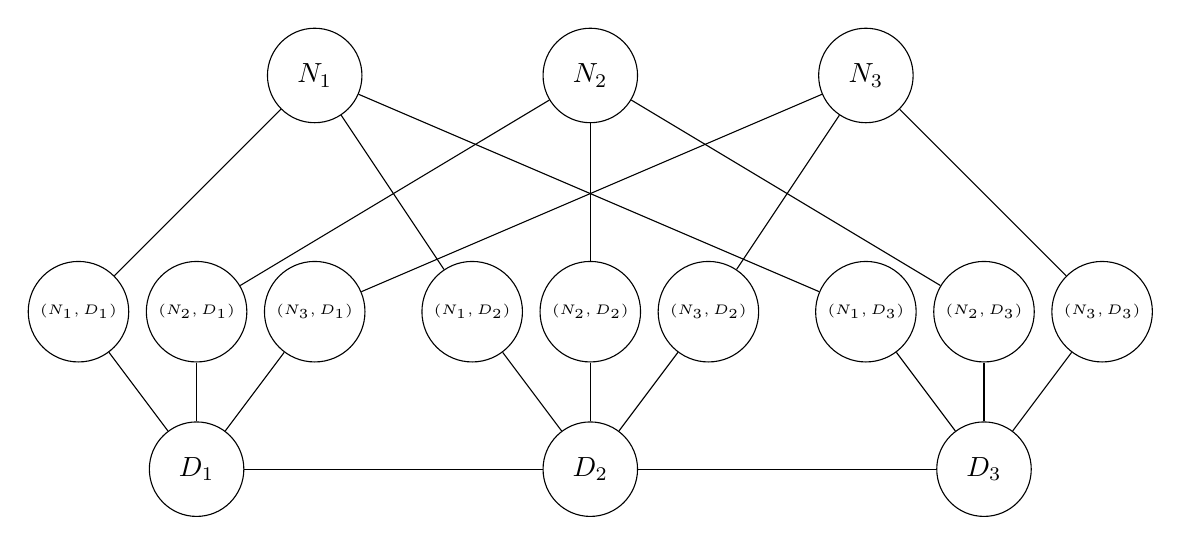
\begin{tikzpicture}[
    				annot/.style={text width=3em, text centered},
    				neuron/.style={circle, draw, minimum size=12mm}]
    				% employee nodes
    				\node[neuron] (n1) at (4, 0) {$N_1$};
    				\node[neuron] (n2) at (7.5, 0) {$N_2$};
    				\node[neuron] (n3) at (11, 0) {$N_3$};
    				% assignment nodes
    				\node[neuron] (n1d1) at (1, -3) {\tiny $(N_1,D_1)$};
    				\node[neuron] (n2d1) at (2.5, -3) {\tiny $(N_2,D_1)$};
    				\node[neuron] (n3d1) at (4, -3) {\tiny $(N_3,D_1)$};
    				\node[neuron] (n1d2) at (6, -3) {\tiny $(N_1,D_2)$};
    				\node[neuron] (n2d2) at (7.5, -3) {\tiny $(N_2,D_2)$};
    				\node[neuron] (n3d2) at (9, -3) {\tiny $(N_3,D_2)$};
    				\node[neuron] (n1d3) at (11, -3) {\tiny $(N_1,D_3)$};
    				\node[neuron] (n2d3) at (12.5, -3) {\tiny $(N_2,D_3)$};
    				\node[neuron] (n3d3) at (14, -3) {\tiny $(N_3,D_3)$};
    				% day nodes
    				\node[neuron] (d1) at (2.5, -5) {$D_1$};
    				\node[neuron] (d2) at (7.5, -5) {$D_2$};
    				\node[neuron] (d3) at (12.5, -5) {$D_3$};
    				% assigned to relations
    				\draw (n1) -- (n1d1);
    				\draw (n1) -- (n1d2);
    				\draw (n1) -- (n1d3);
    				\draw (n2) -- (n2d1);
    				\draw (n2) -- (n2d2);
    				\draw (n2) -- (n2d3);
    				\draw (n3) -- (n3d1);
    				\draw (n3) -- (n3d2);
    				\draw (n3) -- (n3d3);
    				% on day relations
    				\draw (d1) -- (n1d1);
    				\draw (d2) -- (n1d2);
    				\draw (d3) -- (n1d3);
    				\draw (d1) -- (n2d1);
    				\draw (d2) -- (n2d2);
    				\draw (d3) -- (n2d3);
    				\draw (d1) -- (n3d1);
    				\draw (d2) -- (n3d2);
    				\draw (d3) -- (n3d3);
    				% is before relation
    				\draw (d1) -- (d2);
    				\draw (d2) -- (d3);
    		\end{tikzpicture}}
    	\onslide<2>\centering \includegraphics[width=\linewidth, page=3]{figures/graphics.pdf}
    	\end{overprint}
    	\caption{Simplified representation of the destroy set model architecture.}
    \end{figure}
\end{frame}


\begin{frame}{Features }
	\footnotesize
	\structure{For each assignment $(n, d)$}
	\begin{itemize}
		\item flag indicating whether employee $n$ is assigned to shift $s \in S$ on day $d$  
		\item flag indicating whether employee $n$ is assigned to shift $s \in S$ on day $d$ in the original roster 
		\item flag indicating whether employee $n$ is absent on shift $s \in S$ on day $d$  
		\item flag indicating whether the minimum number of consecutive working days constraint is violated for employee $n$ on day $d$
		\item flag indicating whether the maximum number of consecutive working days constraint is violated for employee $n$ on day $d$  
		\item flag indicating whether the minimum number of consecutive assignment constraint is violated for employee $n$ on day $d$ and shift $s \in S$  
		\item flag indicating whether the maximum number of consecutive assignment constraint is violated for employee $n$ on day $d$ and shift $s \in S$  
	\end{itemize}
\end{frame}

\begin{frame}{Features}
	\footnotesize
	\structure{For each employee $n$}
	\begin{itemize}
		\item total number of working assignments of employee $n$  
		\item total number of working assignments of employee $n$ minus minimum number of working days in the planning horizon ($\alpha_{\min}$) 
		\item maximum number of working days in the planning horizon ($\alpha_{\max}$) minus total number of working assignments of employee $n$ 
		\item total number of assignments to shift $s \in S$ of employee $n$ 
		\item total number of assignments to shift $s \in S$ of employee $n$ minus minimum allowed number of assignments to this shift $s$ ($\gamma^{\min}_s$)  
		\item maximum allowed number of assignments to shift $s \in S$ ($\gamma^{\max}_s$) minus total number of assignments to this shift $s$ of employee $n$  
		\item total number of whole day absences of employee $n$
		\item total number of absences per shift $s \in S$ of employee $n$  
	\end{itemize}

	\medskip
	\structure{For each Day $d$}
	\footnotesize
	\begin{itemize}
		\item total number of assignments to each shift $s \in S$ on day $d$  
		\item total number of assignments to each shift $s \in S$ on day $d$ minus cover requirements for this shift $s$ on day $d$ ($R^\text{c}_{ds}$)  
	\end{itemize}
\end{frame}

\begin{frame}{Learning-Based Destroy Operator}
	\framesubtitle{Destroy Set Sampling Strategy}
	\begin{itemize}
		\item Based on \important{consecutive day} observation
		\item Use \important{GNN} outputs $\mu_{nd}$ $\forall n \in N, d \in D$ for refined sampling
	\end{itemize}
	\begin{figure}
		\begin{overprint}
			\onslide<1>\centering\includegraphics[width=\textwidth, page=17]{figures/graphics.pdf}
			\onslide<2>\centering\includegraphics[width=\textwidth, page=18]{figures/graphics.pdf}
			\onslide<3>\centering\includegraphics[width=\textwidth, page=19]{figures/graphics.pdf}
			\onslide<4>\centering\includegraphics[width=\textwidth, page=20]{figures/graphics.pdf}
			\onslide<5>\centering\includegraphics[width=\textwidth, page=21]{figures/graphics.pdf}
			\onslide<6>\centering\includegraphics[width=\textwidth, page=22]{figures/graphics.pdf}
			\onslide<7>\centering\includegraphics[width=\textwidth, page=23]{figures/graphics.pdf}
			\onslide<8,9>\centering\includegraphics[width=\textwidth, page=24]{figures/graphics.pdf}
			%\onslide<10>\centering\includegraphics[width=\textwidth, page=25]{figures/graphics.pdf}
		\end{overprint}
		\caption{Destroy set sampling strategy.}
	\end{figure}
	\onslide<9->\begin{itemize}
		\item Regulate \important{influence} of GNN with \important{temperature} $\tau$
		\begin{itemize}
			\item Such that $\mu_{nd}^\frac{1}{\tau}$ $\forall n \in N, d \in D$
			\item So far $\tau=1$
		\end{itemize}
	\end{itemize}
\end{frame}

\begin{frame}{Learning-Based Destroy Operator}
	\framesubtitle{Temperature Model}
	\begin{itemize}
		\item \important{Learn} temperature $\tau$ for each state with a GNN
		\item \textbf{Input:} 
		\begin{itemize}
			\item graph representation of \important{current solution}
			\item destroy set model \important{outputs}
		\end{itemize}
		%graph representation of current solution,  destroy set model outputs
		\item \textbf{Output:} \important{probabilities} for selecting temperature in $\mathcal{T} = \{ 0.1, 0.2, 0.3, 0.4, 0.5, 0.6, 0.7, 0.8, 0.9, 1, 2, 3, 5 \}$
	\end{itemize}
	\begin{figure}
		\centering\includegraphics[width=\textwidth, page=5]{figures/graphics.pdf}
		\caption{Simplified representation of  the temperature model architecture.}
	\end{figure}
\end{frame}

\begin{frame}{Learning-Based Destroy Operator}
    \framesubtitle{Training}
	\begin{itemize}
		\itemsep 2ex
		\item Offline with representative problem instances via \important{imitation learning}
		\item \important{Expert policy:}\\
		MILP with local branching constraint to determine optimal destroy set
		\item \important{Loss function}: log-likelihood of expert actions,\\
		cross-entropy for temperature
		\item \important{DAGGER \citep{ross2011reduction}}:\\
		Trajectories are first created with expert strategy,\\
		later with learned model
	\end{itemize}
\end{frame}




\begin{frame}{Computational Results}
	\begin{itemize}
		\item Model trained with $|N| = 110$
		%\item LNS time limit of \structure{$15$ minutes}
		\item \structure{MILP + Gurobi} optimality gap between \textbf{26\%} and \textbf{34\%}
	\end{itemize}
	\begin{figure}
		\scalebox{1}{\includegraphics[width=0.5\textwidth]{figures/generalization-box.pdf}\includegraphics[width=0.5\textwidth]{figures/generalization-line.pdf}}
		\caption{Comparison of LNS\_RND and LNS\_NN optimality gaps. $15$ minutes running time. Lower bounds from solving MILP for three hours.}
	\end{figure}
\end{frame}


\begin{frame}
	\frametitle{Conclusions}
	\begin{itemize}
		\itemsep2.5ex
		\item Large variety of ML-based approaches to support/improve metaheuristics
		\item Modern RL techniques seem particularly promising
		\begin{itemize}
			\item to reduce effort in manually crafting/tuning heuristics
			\item without labeled training data (supervised learning)
		\end{itemize}
		\item Naive application of an RL agent to a COP usually not competitive
		\item Combinations with tree search, local search and problem-specific heuristics can boost performance substantially
		\item Keep in mind: 
		\begin{itemize}
			\item (deep) neural networks not always necessary,\\
			e.g., other ML models may be faster \& more robust
			\item deep RL can be tricky
		\end{itemize}
	
	\end{itemize}
\end{frame}





\begin{frame}[allowframebreaks]
	\frametitle{References}
	\footnotesize
	%\nocite{*}
	% \bibliographystyle{abbrv}
	\bibliographystyle{apalike}
	\bibliography{lit.bib}
\end{frame}


\end{document}

\begin{frame}{Speeding up Logic-Based Benders Decomposition by Strengthening Cuts with Graph Neural Networks}
\begin{itemize}
  \itemsep2ex
  \item Work mainly done during a research visit at Linköping University, Sweden,\\ ELIIT Focus Period ``Hybrid AI: Where data-driven and model-based methods meet''

  \item Presented at the 9th Int.\ Conference on Machine Learning, Optimization, and Data Science (LOD) 2023, Grasmere, UK, September, 2023

  \item Article to appear in:\\
  J.\ Varga, E.\ Karlsson, G.\ R.\ Raidl, E.\ Rönnberg, F.\ Lindsten, T.\ Rodemann:\\
  Machine Learning, Optimization, and Data Science -- LOD 2023,
  Revised Selected Papers, Springer.
\end{itemize}
\end{frame}



\section{Logic-based Benders Decomposition}

\begin{frame}{Classical Benders Decomposition}

(\emph{Benders, 1962})

\bigskip
\begin{itemize}
  \itemsep1.5ex
  \item Prominent exact technique for solving large \important{mixed-integer linear programs (MILPs)}
  \item Breaks down MILP into \important{master} and \important{subproblems}
  \item Master problem (MP) considers only subset of variables/constraints
  \item Solving subproblems (SPs):\\
  via duality we obtain \important{Benders feasibility and/or optimality cuts} for MP
  \item Iterative process
  \item<2> \alert{SPs must be linear programs (LPs), only continuous variables allowed}
\end{itemize}
\end{frame}

\begin{frame}{Logic-Based Benders Decomposition}

\emph{J.\ N.\ Hooker and G.\ Ottosson: Logic-based Benders decomposition. Mathematical Programming, 96:33--60, 2003}

\bigskip
\begin{itemize}
  \itemsep1.5ex
  \item Generalization to essentially \important{arbitrary SPs also incl.\ integral variables}
  \item Unfortunately, \alert{no general systematic way of deriving (strong) Benders cuts} exist anymore
  \item Typically, \important{problem-specific cut-strengthening techniques} are applied,\\ exploiting problem structure
\end{itemize}

\bigskip
\structure{Also related:}
\begin{itemize}
  \item Branch and check (\emph{Hooker and Ottosson, 2003})\\
  MP only solved once, SPs when feasible solutions are encountered
  \item \emph{G.~Codato and M.~Fischetti: Combinatorial Benders cuts for mixed-integer linear programming. Operations Research, 54:756--766, 2006} \nocite{2006_codato-fischetti_article}
\end{itemize}


\end{frame}

\begin{frame}
  \frametitle{Logic-based Benders Decomposition}
  \begin{centering}
    \only<1>{
      \includegraphics[width=\textwidth]{img/lbbd1}
    }\only<2>{
      \includegraphics[width=\textwidth]{img/lbbd2}
    }
  \end{centering}

  We consider here only feasibility cuts.

  \bigskip
  \uncover<2>{
    Our approach: \important{Learn strengthening procedure}
  }
\end{frame}


\begin{frame}
  \frametitle{Test bed: Single-Machine Scheduling Problem \footfullcite{2020_horn-et-al_article}}
  \begin{minipage}{0.5\textwidth}
    \begin{itemize}
      \item \important{Single machine}
      \item \important{Tasks} with \important{multiple time windows}
      \item \important{Setup times} between tasks
      \item \important{Prize} for each task
      \item Objective: Maximize \important{total prize} of scheduled tasks
    \end{itemize}
    \vspace{1em}
    \uncover<2->{
      \begin{itemize}
        \item \important{MP:} Select \important{task time window pairs} (TTWP)
        \item \important{SP:} Feasible schedule?
        \item \important{Feasibility cut:} $\widehat{=}$ set of TTWPs
        \item \important{Cut-strengthening:} reduce set
      \end{itemize}
    }
  \end{minipage}%
  \begin{minipage}{0.5\textwidth}
    \scalebox{0.3}{
      \begin{tikzpicture}
        \node at (2,0) {\includegraphics[height=4cm]{img/machine.pdf}};
        \node[rectangle,fill=black!70,minimum width=15cm,minimum height=2cm] at (13.5,0) {};

        \draw[very thick, draw=black] (6,1.5) to (6,-10.5);
        \draw[very thick, draw=black] (21,1.5) to (21,-10.5);

        \node[rectangle,fill=black!40,minimum width=2cm,minimum height=2cm] at (1,-4) {};
        \only<3,4>{\node[rectangle,fill=rgreen,minimum width=4cm,minimum height=2cm] at (9,-4) {};}
        \node[rectangle,draw=black,minimum width=4cm,minimum height=2cm] at (9,-4) {};
        \node[rectangle,draw=black,minimum width=3cm,minimum height=2cm] at (16.5,-4) {};

        \node[rectangle,fill=black!40,minimum width=4cm,minimum height=2cm] at (2,-7) {};
        \only<3,4>{\node[rectangle,fill=rgreen,minimum width=6cm,minimum height=2cm] at (9,-7) {};}
        \node[rectangle,draw=black,minimum width=6cm,minimum height=2cm] at (9,-7) {};
        \node[rectangle,draw=black,minimum width=5cm,minimum height=2cm] at (18.5,-7) {};

        \node[rectangle,fill=black!40,minimum width=3cm,minimum height=2cm] at (1.5,-10) {};
        \only<3>{\node[rectangle,fill=rgreen,minimum width=3cm,minimum height=2cm] at (10.5,-10) {};}
        \node[rectangle,draw=black,minimum width=3cm,minimum height=2cm] at (10.5,-10) {};
        \node[rectangle,draw=black,minimum width=3cm,minimum height=2cm] at (16.5,-10) {};
      \end{tikzpicture}
    }
  \end{minipage}
\end{frame}

\begin{frame}{Cut Strengthening Methods}

\structure{Deletion filter:}
\begin{itemize}
  \item Consider TTWPs iteratively and try to remove each
  \item Accept removal when subproblem remains infeasible
  \item $\rightarrow $ \important{irreducible set of TTWPs / cut}
  \item Order of TTWPs is crucial, but ``best'' order unknown!
\end{itemize}

\bigskip
\structure{MARCO (Liffiton and Malik, 2013):}
\begin{itemize}
  \item Enumerates \important{\emph{all} irreducible sets of TTWPs} systematically
  \item Much more expensive in terms of SPs to check
\end{itemize}

\bigskip 
%\emph{Karlsson and Rönnberg (2021):} Comparison of different cut strengthening procedures\nocite{karlsson2021strengthening}
\fullcite{karlsson2021strengthening}

\bigskip
Our approach: based on the faster deletion filter,\\
but for obtaining training data we use MARCO.
\end{frame}


\section{Learning the Strengthening of Cuts}

\begin{frame}
  \frametitle{GNN-Based Cut-Strengthening}
  Learn \important{Graph Neural Network (GNN) based function}
  \begin{equation*}
    f_\Theta(
      \,\overbrace{I}^\text{\hspace{-1cm}instance\hspace{-1cm}}\,,
      \,\underbrace{X}_\text{\hspace{-1cm}TTWPs from MP\hspace{-1cm}}\,,
      \,\overbrace{S}^\text{\hspace{-1cm}selected TTWPs\hspace{-1cm}}\,
    )
    \qquad \longrightarrow \qquad
    \underbrace{(i,w)}_\text{next TTWP to add to $S$} \text{ and }\quad
    \underbrace{\tau}_\text{stop?}
  \end{equation*}

  \bigskip
  \uncover<2->{
    \noindent\important{Given:} problem instance $I$, feasibility cut $X$ \\
    \important{Return:} strengthened feasibility cut
    \begin{enumerate}
      \item Start with $S=[]$
      \item Autoregressively add TTWPs $(i,w)$ until $\tau$
      \item Autoregressively add TTWPs $(i,w)$ until subproblem($S$) is infeasible
      \item Apply deletion filter in reverse order of $S$
    \end{enumerate}
  }
\end{frame}

\begin{frame}
  \frametitle{GNN Architecture\footnote{Inspired by \fullcite{kool2019attention}}}
  Complete directed graph with nodes $\widehat{=}$ \important{$X$} (TTWPs from MP solution) \\
  \important{Input:} 16 node features $x$, 7 arc features $y$ \\
  \important{Output:} $p$, $\tau$

  \begin{centering}
    \scalebox{0.7}{
      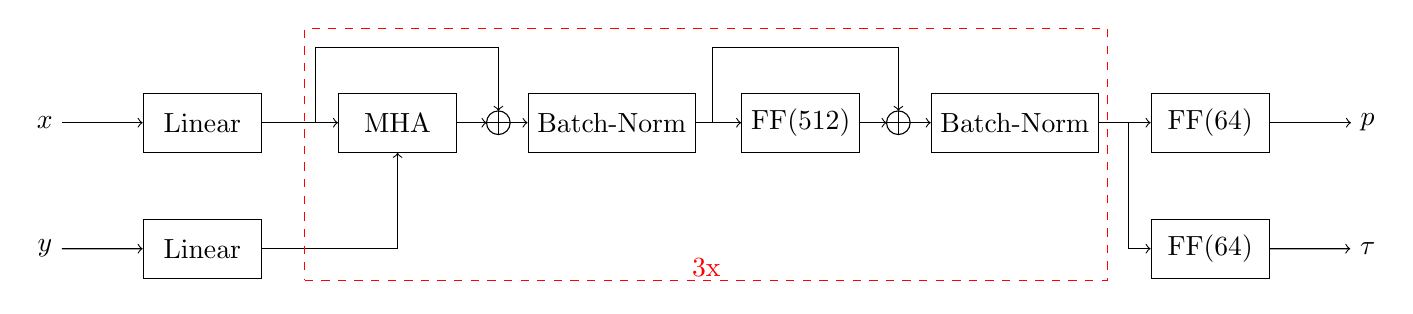
\begin{tikzpicture}[scale=0.8]
        \node at (0,0) (x) {$x$};
        \node[layer] at (2.5,0) (linx) {Linear};
        \node at (0,-2) (y) {$y$};
        \node[layer] at (2.5,-2) (liny) {Linear};
        \node[layer] at (5.6,0) (mha) {MHA};
        \node[plus] at (7.2,0) (skip-mha) {};
        \node[layer] at (9,0) (bn-mha) {Batch-Norm};
        \node[layer] at (12,0) (ff) {FF(512)};
        \node[plus] at (13.55,0) (skip-ff) {};
        \node[layer] at (15.4,0) (bn-ff) {Batch-Norm};
        \node[layer] at (18.5,0) (ffp) {FF(64)};
        \node at (21,0) (p) {$p$};
        \node[layer] at (18.5,-2) (fff) {FF(64)};
        \node at (21,-2) (f) {$\tau$};

        \draw[->] (x) -- (linx);
        \draw[->] (linx) -- (mha);
        \draw[->] (y) -- (liny);
        \draw[->] (liny) -| (mha);
        \draw[->] (mha) -- (skip-mha);
        \draw[->] (linx) -| ++(1.8,1.2) -| (skip-mha);
        \draw[->] (skip-mha) -- (bn-mha);
        \draw[->] (bn-mha) -- (ff);
        \draw[->] (ff) -- (skip-ff);
        \draw[->] (bn-mha) -| ++(1.6,1.2) -| (skip-ff);
        \draw[->] (skip-ff) -- (bn-ff);
        \draw[->] (bn-ff) -- (ffp);
        \draw[->] (ffp) -- (p);
        \draw[->] (bn-ff) ++(1.8,0) |- (fff);
        \draw[->] (fff) -- (f);

        \node[rectangle, draw=red, dashed, minimum width=10.2cm, minimum height=3.2cm] at (10.5,-0.5) {};
        \node[text=red] at (10.5, -2.3) {3x};
      \end{tikzpicture}
    }
    \captionof{figure}{Architecture of the GNN.}
  \end{centering}

  \important{MHA:} Multi-head attention, i.e., transformer-based convolution layer with 8 heads

  \bigskip
  $f_\Theta$ returns TTWP with maximal $p$ and rounded $\tau$
\end{frame}

\begin{frame}
  \frametitle{Training}
  Offline, in supervised fashion using representative problem instances

  \bigskip
  \structure{Collecting training samples:}

  \medskip
  \begin{enumerate}
    \itemsep2ex
    \item \important{Run Logic-based Benders Decomposition}
      \begin{itemize}
        \item enumerate \important{\emph{all} irreducible cuts} via MARCO, add them to the MP
        \item record all SPs and cuts
      \end{itemize}
    \item Determine a minimal subset of \important{\bf strong cuts},\\
      i.e., cuts actually required in MP to get feasible optimal solution
    \item For each subproblem: \important{Rollouts}
      \begin{itemize}
        \item Start with empty set $S$
        \item Successively add TTWPs leading to a strong cut randomly until $S$ $\widehat{=}$ irreducible cut
        \item \important{Each iteration:} add \important{training sample}
        \item \important{Labels:} based on strong cuts
      \end{itemize}
  \end{enumerate}

  \bigskip
  Loss function: binary cross-entropy
\end{frame}

\section{Results}

% \begin{frame}[fragile]
%   \frametitle{Experiments Setup}
%   \begin{itemize}
%     \item \important{Instances} like in \emph{Horn, Raidl, and Rönnberg (2021)}, $n\in\{10,15,20,25\}$ tasks
%     \item \verb|pytorch_geometric|, Gurobi 9.5, CP\,Optimizer 20.1
%     \item AMD Ryzen 9 5900X
%     \item For each $n$: 300\,000 to 600\,000 training samples from 2.000 to 200\,000 instances
%     \item 40 to 300 training epochs
%     \vspace{6mm}
%     \item Comparison to \important{deletion filter} with different orders:
%       \begin{itemize}
%         \item Random
%         \item Sorted: natural order from instance
%         \item Hooker \footfullcite{2013_coban-hooker_article}: sorted by decreasing slack
%       \end{itemize}
%   \end{itemize}
% \end{frame}

% \begin{frame}
%   \frametitle{Results: Number of Solved SPs to Reach Optimality}
%   \centering
%   \cumuldistr{../lod23/csv/avionics20_inst20}{no_subproblems_performed}{0.8\textwidth}{0.6\textheight}{\# of solved subproblems}{\# of solved\\instances}{\normalsize 20 Tasks}
%   \ref{legend:cumuldistr-../lod23/csv/avionics20_inst20-no_subproblems_performed}

%   \bigskip
%   Reduction: $\approx 70\%$
% \end{frame}

% \begin{frame}
%   \frametitle{Results: Time to Reach Optimality}
%   \centering
%   \cumuldistr{../lod23/csv/avionics20_inst20}{time_spent}{0.8\textwidth}{0.6\textheight}{Time {[s]}}{\# of solved\\instances}{}\hfill
%   \ref{legend:cumuldistr-../lod23/csv/avionics20_inst20-time_spent}

%   \bigskip
%   Reduction: $\approx 50\%$
% \end{frame}

% \begin{frame}
%   \frametitle{Results: Number of MP Iterations}
%   \centering
%   \cumuldistr{../lod23/csv/avionics20_inst20}{no_benders_iteration}{0.8\textwidth}{0.6\textheight}{Time {[s]}}{\# of LBBD iterations}{}\hfill
%   \ref{legend:cumuldistr-../lod23/csv/avionics20_inst20-no_benders_iteration}
% \end{frame}

% \begin{frame}{Results: Bounds over Time}
%   \centering
%   \includegraphics[width=10cm]{img/results-bounds.png}\hfill
%   \ref{legend:cumuldistr-../lod23/csv/avionics20_inst20-no_benders_iteration}
% \end{frame}

% \begin{frame}{Results: Out-of-Distribution Usage of GNNs}
%   \centering
%   25 Tasks\\
%   \includegraphics[width=15cm]{img/results-extrapolation.png}
% \end{frame}

% \section{Conclusion}

% \begin{frame}
%   \frametitle{Conclusion and Future Work}
%   \begin{itemize}
%     \itemsep1.5ex
%     \item \important{GNN} to \important{guide cut strengthening} in Logic-based Benders Decomposition
%     \item Reduced \# subproblems to be solved by $\approx 70\%$
%     \item Reduced runtime by $\approx 50\%$
%     \item Promising future work
%       \begin{itemize}
%         \item Application to other/more complex problems
%         \item Deeper analysis of importance of features, GNN structure
%         \item Curriculum learning
%         \item Reinforcement learning
%       \end{itemize}
%   \end{itemize}
% \end{frame}

% \part{End}

% \begin{frame}
%   \frametitle{}
%   \centering
%   \LARGE
%   Thank you!

%   \vspace{1em}
%   Paper to appear in LOD~23 post-conference proceedings:\\
%   \includegraphics[width=0.3\textwidth]{img/qrcode.pdf}
% \end{frame}

%\appendix

\section{References}

% ### Bibliography ################################################################################
\begin{frame}%[allowframebreaks]
  \frametitle{References}
  \nocite{saken2023computational}
  \printbibliography
\end{frame}

\section{Backup}

\begin{frame}{Node Features}
  \centering
  \includegraphics[height=0.9\textheight]{img/node-features.png}
\end{frame}

\begin{frame}{Arc Features}
  \centering
  \includegraphics[height=0.65\textheight]{img/arc-features.png}
\end{frame}

\end{document}
